%\RequirePackage{lineno}
\documentclass[aps,prc,preprint,superscriptaddress,showpacs,showkeys]{revtex4-1}
\usepackage{graphicx}
\begin{document}
\newcommand{\Jpsi}{J/\psi}
\newcommand{\pT}{p_{T}}

%\linenumbers
\title{{\Large Quarkonia suppression in PbPb collisions at $\sqrt s_{NN}$ =  2.76 TeV }}
\author{\large Vineet Kumar}
\author{\large Prashant Shukla}
\email{pshukla@barc.gov.in}
\affiliation{Nuclear Physics Division, Bhabha Atomic Research Center, Mumbai, India}
\affiliation{Homi Bhabha National Institute, Anushakti Nagar, Mumbai, India}
\author{\large Ramona Vogt}
\affiliation{Physics Division, Lawrence Livermore National Laboratory, Livermore, CA 94551, USA}
\date{\today}

\begin{abstract}
  We estimate the modification of quarkonia yields in the medium produced in PbPb
collisions at LHC energy. A kinetic model is employed which incorporates quarkonia  
suppression inside QGP, suppression due to hadronic comovers and 
regeneration from charm pairs.
 Quarkonia dissociation cross section due to gluon collisions has been considered and
the regeneration rate has been obtained using the principle of detailed balance.
Modification in yield due to change in parton distribution functions inside nucleus and 
due to collisions with comovers has been estimated assuming it to be caused by pion.  
  The menifestations of these effects in different kinematic regions in
the nuclear modification factors for both $\Jpsi$ and $\Upsilon$ has been studied
in PbPb collisions at $\sqrt s_{NN}$ =  2.76 TeV. 
  Both the suppression and regeneration due to deconfined medium strongly affect 
low $\pT$ range. The large observed suppression of $\Jpsi$ at high $p_T$ far exceeds
the estimates of suppression by deconfine medium.
\end{abstract}

\pacs{12.38.Mh, 24.85.+p, 25.75.-q}
\keywords{quark-gluon plasma, quarkonia, suppression, regeneration}
\maketitle
%%%%%%%%%%%%%%%%%%%%%%%%%%%%%%%%%%%%%%%%%%%%%%%%%%%%%%%%%%%%%%%%%%%%%%%%%%%%%%%%%%%%%%%%%%%%%%%%%%%%%%%%%%%%%%%%%
\section{Introduction}
  Heavy ion collisions at relativistic energies are performed to create and characterize 
Quark Gluon plasma (QGP), a phase of strongly interacting matter at high energy density 
where quarks and gluons are no longer bound within hadrons. 
  Quarkonia state ($\Jpsi$ and $\Upsilon$) have been one of the most popular tools 
since their suppression was proposed as a signal of QGP \cite{Matsui:1986dk}.
  The understanding of these probes has evolved substantially via measurements 
through three generations of experiments: SPS (at CERN), RHIC (at BNL) and the LHC (at CERN) 
and by voluminous theoretical activities [For recent reviews see 
Refs.~\cite{Schukraft:2013wba,Kluberg:2009wc,Brambilla:2010cs}].
Quarkonia are produced early in the heavy ion collisions and if they evolve
through deconfined medium their yields should be suppressed in comparison with those in $pp$. 
 The first such measurement was the 'anomalous' $\Jpsi$ suppression discovered at the SPS 
which was considered as a hint of QGP formation. The RHIC measurements showed almost the 
same suppression at a much higher energy contrary to the expectation \cite{Brambilla:2010cs,Adare:2011yf}. 
 Such an observation was consistent with the scenarios that at higher collision energy the 
expected more suppression is compensated by regeneration of $\Jpsi$ by recombination of two 
independently produced charm quarks~\cite{Andronic:2003zv}.
After the LHC started PbPb collisions at $\sqrt s_{NN} = 2.76$ TeV, a wealth of
results have become available on quarkonia production \cite{Muller:2012zq,P.ShuklaforCMS:2014vna}. 
  The CMS experiment carries out $\Jpsi$ measurement at high transverse momentum 
($p_T>6.5$ GeV/$c$). The nuclear modification factor  $R_{AA}$ of these high $p_T$ 
prompt $\Jpsi$ decreases with increasing centrality \cite{Chatrchyan:2012np,Mironov:2013jaa} showing
moderate suppression even in the most peripheral collisions. 
  Moreover $R_{AA}$ is found to be nearly independent of $p_T$ (above 6.5 GeV$/c$) showing 
that $\Jpsi$ remain suppressed even at very high $p_T$ upto 16 GeV/$c$.
 On comparing with the STAR results \cite{Tang:2011kr} at RHIC it follows that the suppression of
(high $p_T$) $\Jpsi$ has increased with collision energy.
  The ALICE results \cite{Abelev:2013ila} of $\Jpsi$ covers low $p_T$ range which
have little or no centrality dependence. The ALICE $\Jpsi$ suppression decrease 
substantially with decreasing $p_T$ and at very low $p_T$ the suppression is small.
  When compared with PHENIX forward rapidity measurement at 
RHIC \cite{Adare:2011yf}, it suggests that low p$_T$ $\Jpsi$ are less suppressed at LHC.
 These observations suggest regeneration of $\Jpsi$ at low $p_T$ by 
recombination of independently produced charm pairs.
  The CMS measurements \cite{Chatrchyan:2011pe,Chatrchyan:2012lxa} reveal that 
the higher $\Upsilon$ states are more suppressed relative to the ground state, 
a phenomenon known as sequential suppression. The ALICE
 measurements in forward rapidity ($2.5 \leq y^{\Upsilon} \leq 4.0$) are 
consistent with CMS measurements in mid rapidity region ($|y^{\Upsilon}|\,\leq 2.4$).

 Many theoertical frameworks have been developed in pre-LHC years for the modification of 
quarkonia due to different processes. 
 The suppression of quarkonia in QGP are understood in terms of colour screening models  
e.g. Ref. \cite{Matsui:1986dk,Abdulsalam:2012bw}and alternatively in terms of dissociation of quarkonia 
by gluon collision process \cite{Bhanot:1979vb,Xu:1995eb}. The statistical models \cite{Andronic:2003zv,Andronic:2012dm}
offer estimates of the regeneration of quarkonia from charm quark pairs.
The inverse of gluon dissociation process is also used to estimate regeneration \cite{Thews:2000rj}.  
  The quarkonia yields in heavy ion collisions are also modified due to non-QGP effects such as
shadowing, an effect due to change of the parton distribution functions inside the nucleus,
and dissociation due to hadronic or comover interaction \cite{Vogt:2010aa}.
 There have been many recent calculations to explain the LHC results on quarkonia using a 
combination of above theoretical frameworks and models \cite{Zhao:2011cv,Emerick:2011xu}. 

In this paper, we calculate the quarkonia (both $\Jpsi$ and $\Upsilon$) production and
suppression in a kinetic model which includes dissociation due to thermal gluons, modification 
of yield due to change in parton distribution functions inside nucleus and due to collisions with 
comover hadrons. Regeneration by thermal charm pairs is also take into account. 
 Our goal is obtain the nuclear modification factor of quarkonia as a function of transverse 
momentum and centrality of collision to be compared with experimental data from CMS 
and ALICE.

\section{Heavy quark production rates}
The production cross sections for heavy quark pairs are calculated to NLO in pQCD  
using the CTEQ6M parton densities \cite{Pumplin:2002vw,Pumplin:2000vx}.  The central EPS09 parameter set 
\cite{Eskola:2009uj} is used to calculate the modifications of the parton densities in 
PbPb collisions.  We use the same set of parameters
as that of Ref.~\cite{Cacciari:2005rk} with the NLO calculation of Ref.~\cite{Mangano:1991jk}
to obtain the exclusive $Q \overline Q$ pair rates.  
 The production cross sections for heavy flavor and quarkonia at $\sqrt{s_{_{NN}}}= 2.76$ 
TeV \cite{Kumar:2012qx} are given in Table~\ref{NLOcros}.  The number of $Q \overline Q$ pairs
in a minimum bias PbPb event is obtained from the per nucleon cross
section, $\sigma_{\rm PbPb}$, by
\begin{eqnarray}
N_{Q \overline Q} = {A^2 \sigma_{\rm PbPb}^{Q \overline Q}  \over  
\sigma_{\rm PbPb}^{\rm tot}} \, \, .
\end{eqnarray}
 At 2.76 TeV, the total PbPb cross section, $\sigma_{\rm PbPb}^{\rm tot}$, 
is 7.65 b \cite{Chatrchyan:2011sx}.

\begin{table}
\caption[]{Heavy quark and quarkonia production  cross sections at
$\sqrt{s_{_{NN}}}= 2.76$ TeV. The cross sections are given per nucleon pair while
$N$ gives number of heavy quark pair/quarkonia per PbPb event.}
\label{NLOcros}
\begin{tabular}{l|l|l|l|l} 
\hline 
\hline
                     & $ c \overline c$           &$\Jpsi$      & $ b \overline b$           & $\Upsilon$   \\              
\hline
$\sigma_{\rm PbPb}$  & $1.76^{+2.32}_{-1.29}$ mb  & $31.4 \mu$b  & $89.3^{+42.7}_{-27.2} \mu$b  & $0.38 \mu$b  \\
$N$                  &$9.95^{+13.10}_{-7.30}$     & $0.177$      & $0.50^{+0.25}_{-0.15}$     & $0.01$       \\
\hline
\hline
\end{tabular}
\end{table}





%%%%%%%%%%%%%%%%%%%%%%%%%%%%%%%%%%%%%%%%%%%%%%%%%%%%%%%%%%%%%%%%%%%%%%%%%%%%%%%%%%%%%%%%%%
\section{Modification of quarkonia in the presence of QGP}
 In the Kinetic approach \cite{Thews:2000rj}, the proper time ($\tau$) evolution of the $\Jpsi$ population 
is given by the rate equation 

\begin{equation}\label{eqkin}
{dN_{\Jpsi} \over d\tau}  =  - \lambda_D  \rho_g N_{\Jpsi} + \lambda_F {N_{c \bar{c}}^{2} \over V(\tau)},
\end{equation}
where $V(\tau)$ is the volume of the deconfined spatial region and $N_{c \bar{c}}$ is the number of initial 
charm quark pairs produced per event.
 The $\lambda_{D}$ is the dissociation rate obtained by the dissociation cross-section averaged over the momentum 
distribution of gluons and $\lambda_{F}$ is the formation rate obtained by the formation cross-section 
averaged over the momentum distribution of $c$ and $\bar c$. $\rho_g$ is the density of thermal gluons.
 The number of $\Jpsi$ at freeze-out time $\tau_f$ is given by solution of Eq.~(\ref{eqkin}) as
\begin{equation}
N(p_T) = S(p_T) \,N_{\Jpsi}^{0}(p_T)+N_{\Jpsi}^F(p_T).
\label{eqbeta}
\end{equation}
Here $N_{\Jpsi}^{0}(p_T)$ is the number of initially produced $\Jpsi$ as a function of $p_T$ and 
$S(p_T)$ is their survival probability from gluon collisions at freeze-out time $\tau_f$ and 
is written as
\begin{equation}
S(\tau_f,p_T) = \exp \left( {-\int_{\tau_0}^{\tau_f}f(\tau) \lambda_{\rm D}(T,p_T)\,\rho_g(T)\,d\tau} \right).
\end{equation}
The temperature $T(\tau)$ and the QGP fraction $f(\tau)$ evolve from initial time $\tau_0$ to 
freeze-out time $\tau_f$ due to expansion of QGP.
$N_{\Jpsi}^F(p_T)$ is the number of regenerated $\Jpsi$ per event and is given by
\begin{equation}
N_{\Jpsi}^F(p_T)=S(\tau_f,p_T)N_{c \bar{c}}^{2} \int_{\tau_0}^{\tau_f}{{\lambda_{\mathrm{F}}(T,p_T) \over V(\tau)\,S(\tau,p_T)} d\tau}
\end{equation}

   The nuclear modification factor ($R_{AA}$) can be written as 
\begin{equation}
R_{AA}(p_T)=S(p_T) + \frac{N_{\Jpsi}^F(p_T)}{N_{\Jpsi}^{0}(p_T)}
\label{raa}
\end{equation}
$R_{AA}$ as a function of collision centrality, including the regeneration will be  
\begin{equation}
R_{AA}(N_{\rm part}) = \frac{\int_{p_{T\,\rm Cut}} N_{\Jpsi}^{0}(p_T)S(p_T)dp_T}{\int_{p_{T\,\rm Cut}} N_{\Jpsi}^{0}(p_T) dp_T} + 
\frac{\int_{p_{T\, \rm Cut}} N_{\Jpsi}^F(p_T) dp_T}{\int_{p_{T\, \rm Cut}} N_{\Jpsi}^{0}(p_T) dp_T}
\label{raa2}
\end{equation}
Here $p_{\rm Cut}$ defines the $p_T$ range as per the experimental measurements.
 $N_{\Jpsi}^{0}(p_T)$ is the unmodified $p_T$ distribution of $\Jpsi$ obtained by NLO 
calculations which is scaled to a particular centrality of PbPb collisions.

The feed down correction from higher states are also taken into account while calculating
R$_{AA}$ for $\Jpsi$
\begin{equation}
R_{AA}(\Jpsi) = f_{1} \, R_{AA}(\Jpsi) +  f_{2}\, R_{AA}(\psi(2S)) +  f_{3}\, R_{AA}(\chi_{c})
\end{equation}
$f_{1},\,f_{2},\,f_{3}$ are 0.60, 0.08 and 0.32 taken from CDF \cite{Abe:1997yz} and PHENIX measurements 
\cite{Atomssa:2008dn}. Feed down corrections are also applied for $\Upsilon$ states taken from Ref. \cite{Abdulsalam:2012bw}.

The temperature evolution for different centralities of collision is obtained by 
assuming an isentropical cylindrical expansion with volume element
\begin{equation}
V(\tau) = \tau\,\pi\,(R_0 + {1\over 2} a \, \tau^2 )^{2},
\end{equation}
 where a$_T$=0.1c$^2$ fm$^{-1}$ is the transverse acceleration \cite{Zhao:2011cv}.
The initial transverse radius, $R_0$ as a function of centrality is 
obtained in terms of the radius of the Pb nucleus ($R_{\rm Pb}$) as
\begin{equation}
R_0(N_{\rm part}) = R_{\rm Pb} \, \sqrt{N_{\rm part} \over N_{\rm part0} }.
\label{RVsNPart}
\end{equation}
where $N_{\rm part0} $ is the total number of participants in head-on collisions.

The time evolution of temperature is governed by the entropy conservation condition 
$s(\tau)\,V(\tau)= s(\tau_0)\,V(\tau_0)=S_{\rm QGP}$. 
Using $s(\tau)=4a_qT^3$ for entropy density in QGP, the temperature evolution is obtained as
\begin{eqnarray}
\left[T(\tau)\right]^{3} = \frac{S_{\rm QGP}}{4a_qV(\tau)}.
\end{eqnarray}
where $a_{q} = (7N_f/60 + 16/90)\pi^2$ are the degrees of freedom in quark gluon phase.
We relate initial temperature with measured charged particle multiplicity as
\begin{eqnarray}
S_{\rm QGP} = 4a_qV(\tau_0)|_{0-5\%} T_{0}^{3} = a_{\rm m}\left(\frac{dN}{d\eta}\right)_{0-5\%}. 
\label{TempVsMult}
\end{eqnarray}  
Here a$_{\rm m}$ = 5.0 is proportionality factor between charge particle multiplicity and total entropy
of the system \cite{Shuryak:1992wc}. Using $(dN/d\eta)_{0-5\%}$=1.5$\times$1600 obtained from the charge particle 
multiplicity measured in PbPb collisions at 2.76 TeV \cite{Aamodt:2010cz} and N$_f$ = 2.5, we calculate 
initial temperature 0.570 GeV at time $\tau_0$ = 0.2 fm/c.
Transverse size of the system for 0-5$\%$ centrality is $R_{0-5\%}$ = 0.92$R_{\rm Pb}$,
 obtained from Eq.~(\ref{RVsNPart}). 
The initial temperature for different centralities is calculated by 
\begin{equation}
T_{0}^{3}({N_{\rm part}})=T_{0}^{3}\left(\frac{dN/d\eta}{N_{\rm part}/2}\right)/\left(\frac{dN/d\eta}{N_{\rm part}/2}\right)_{0-5\%}
\label{TempNpart}
\end{equation}
  Figure \ref{fig:TauVsTemp} shows time evolution of the temperature and QGP fraction 
in case of most central (0-5$\%$) collisions 
for both longitudinal and cylindrical expansions. The temperature
decreases more rapidily for cylindrical expansion than in case of longitudinal expansion. 
It becomes constant at $T_C$ = 0.170 GeV,  while QGP fraction keeps decreasing. 
Once the hadronization is completed the temperature starts decreasing again till kinetic 
freeze out at temperature $T_f=0.100$ GeV.  


\begin{figure}
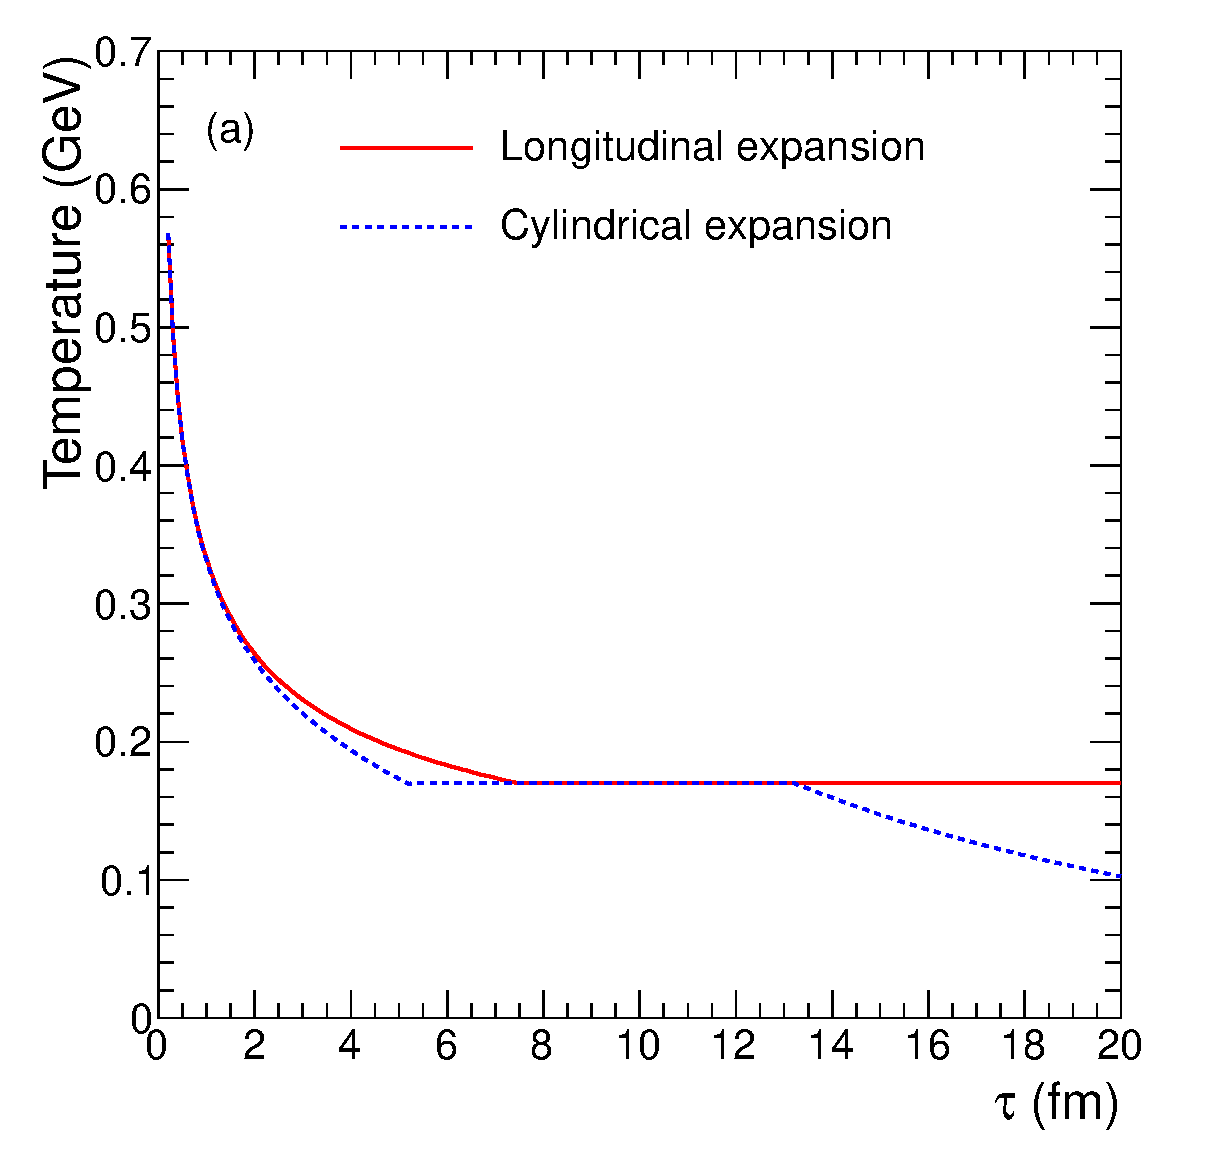
\includegraphics[width=0.49\textwidth]{Figures/Fig1a_TauVsTemp.eps}
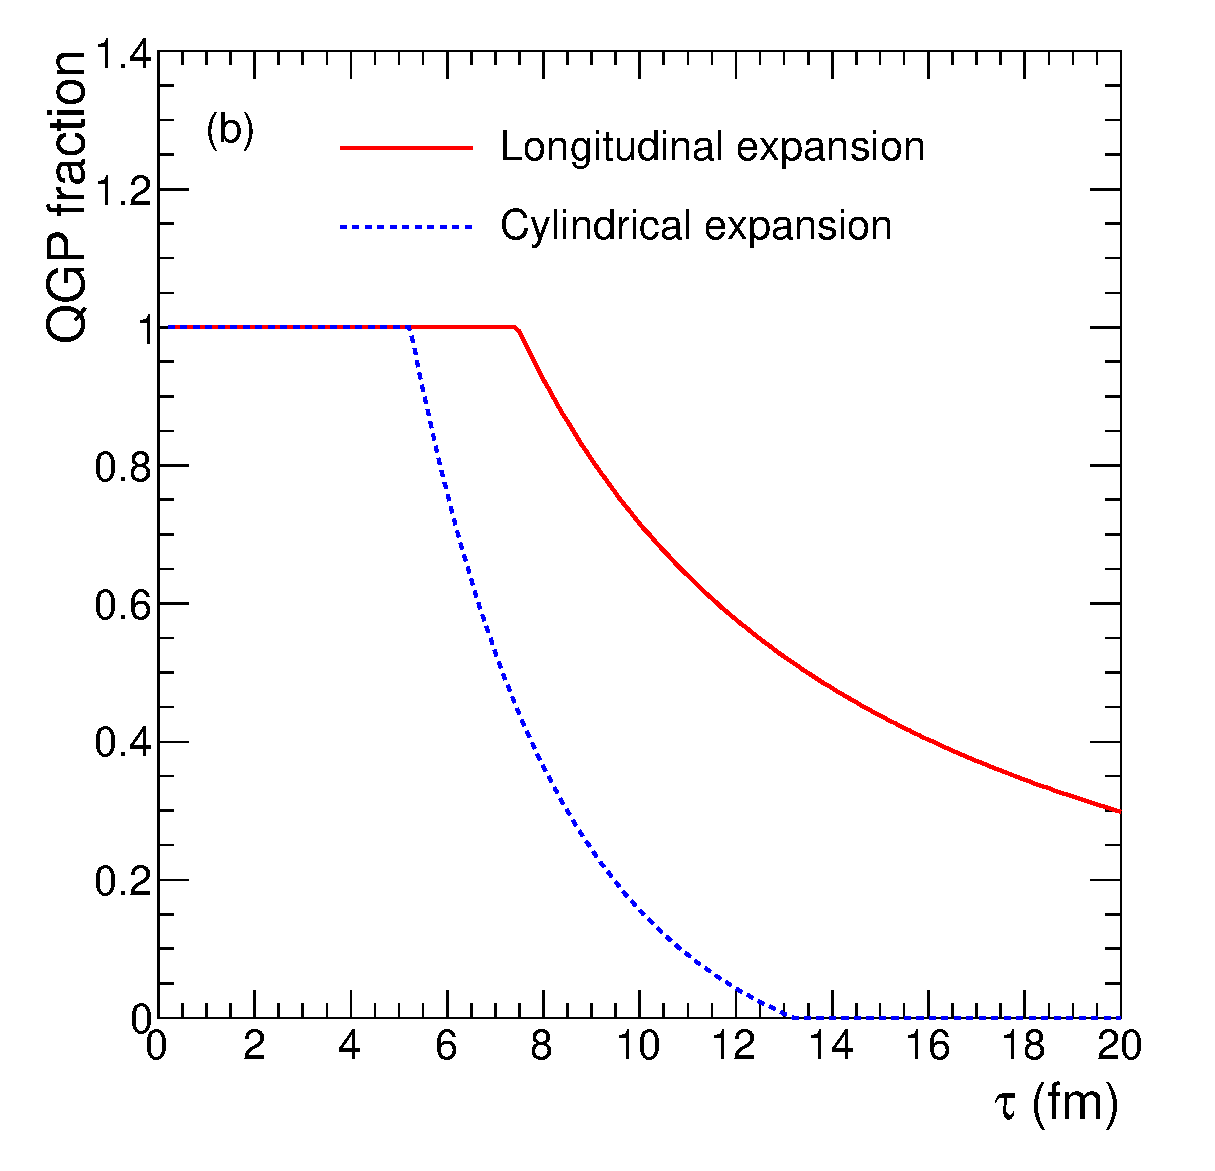
\includegraphics[width=0.49\textwidth]{Figures/Fig1b_TauVsFQGP.eps}
\caption{(Color online) (a) Temperature and (b) QGP fraction in the system as a function of proper 
time in case of most central (0-5$\%$) collisions for longitudinal and cylindrical expansions.}
\label{fig:TauVsTemp}
\end{figure}

%%%%%%%%%%%%%%%%%%%%%%%%%%%%%%%%%%%%%%%%%%%%%%%%%%%%%%%%%%%%%%%%%%%%%%%%%%%%%%%%%%%%%%%%%%%%%%%%%




\begin{table}
\caption[]{Quarkonia properties as predicted by non-relativistic potential model using 
``Cornell'' potential \cite{Karsch:1987pv}.}
\label{Tab:QuarkoniaProperties}
\begin{tabular}{l|l|l|l|l|l|l|l|l} 
\hline   
\hline
    &$\Jpsi$  &$\chi_c$  &$\psi(2S)$ &$\Upsilon(1S)$ &$\chi_b(1P)$ &$\Upsilon(2S)$ &$\chi_b(2P)$ &$\Upsilon(3S)$ \\ 
\hline 
Mass [GeV/$c^2$]                      &3.10     &3.53  &3.68  &9.46  &9.99  &10.02  &10.26   &10.36 \\
Binding Energy $\epsilon_{0}$ [GeV]                  &0.64     &0.20  &0.05  &1.10  &0.67  &0.54   &0.31    &0.20 \\
%Radius [fm]                           &0.25     &0.36  &0.45  &0.14  &0.22  &0.28   &0.34    &0.39 \\
%Formation time $\tau_{\rm Form}$ [fm]    &0.89     &2.0   &1.5   &0.76  &2.6   &1.9    &2.6      &2.4 \\
\hline
\hline
\end{tabular}
\end{table}


\subsection{Dissociation Rate}
   In colour dipole approximation the gluon dissociation cross section as function of gluon energy $q^0$
in the J$/\psi$ rest frame is given by \cite{Bhanot:1979vb}
\begin{equation}
\sigma_{D}(q^{0}) = 4\pi\,\left(\frac{8}{3}\right)^3\,\frac{1}{m_c^{3/2}}\,\epsilon_0^3 \frac{ (q^0-\epsilon_0)^{3/2}}{(q^0)^5},
\end{equation}
where $\epsilon_0$ is the quarkonia binding energy and $m_c$ is the charm/bottom quark mass.
The values of $\epsilon_0$ for different quarkonia states are given in Table~\ref{Tab:QuarkoniaProperties}.
 Figure \ref{fig:SigmaDQ0} shows the gluon dissociation cross section of $\Jpsi$ and $\Upsilon(1S)$
as a function of gluon energy. 
 The dissociation cross section is zero when gluon energy is less than the binding energy
of the $\Jpsi$. It increases with gluon energy and reaches  maximum at 1.2 (1.5) GeV for 
$\Jpsi\,(\Upsilon)$. At higher gluon energy, the interaction probability decreases.
$q^0$ is related to the centre of mass energy $s$, of $\Jpsi$-gluon system as
\begin{eqnarray}
 q^{0} = \frac{s-M_{\Jpsi}^{2}}{2\,M_{\Jpsi}}.
\end{eqnarray}  
  Using this relation $\sigma_{D}(q^0(s))$ can be obtained which we write as $\sigma_{D}(s)$.
The centre of mass energy square $s$ can be obtained as
$s=m_{\Jpsi}^{2} + 2E_{\Jpsi}E_{g}(1-{\rm cos\theta})$,
where $E_g\,(E_{\Jpsi})$ is energy of gluon ($\Jpsi$) and $\theta$ is angle between them.
 
 We can calculate dissociation rate by folding the dissociation cross-section on thermal gluon 
distribution $f_{g}(p)$ as   
\begin{eqnarray}
\lambda_{D} \rho_{g}  & = & \langle \sigma v_{\rm rel} \rangle \,\rho_{g}  = 
      \frac{g_g}{(2\pi)^{3}} \int d^{3}p \, f_{g}(p) v_{\rm rel} \, \sigma_{D}(s)   \nonumber \\ 
& = &\frac{g_g}{(2\pi)^{3}} \int  2\pi p^{2} dp f_{g}(p) \int \sigma_{D}(s) v_{\rm rel}(s) d({\rm cos\theta})  
\end{eqnarray}
 The relative velocity $v_{\rm rel}$ between the $\Jpsi$ and gluon is given by
\begin{eqnarray}
 v_{\rm rel}  = {s- M_{\Jpsi}^{2} \over 2E_{\Jpsi}E_{g}}  
\label{eq7}
\end{eqnarray}

 Figure \ref{fig:DRateVsTempAndPt} shows  gluon dissociation rate for $\Jpsi$ as a 
function of medium temperature and $\Jpsi$ transverse momentum. Dissociation rate increases 
with temperature due to increase in gluon density. Dissociation rate of $\Jpsi$ is maximum 
at rest and decreases with transverse momentum.


\begin{figure}
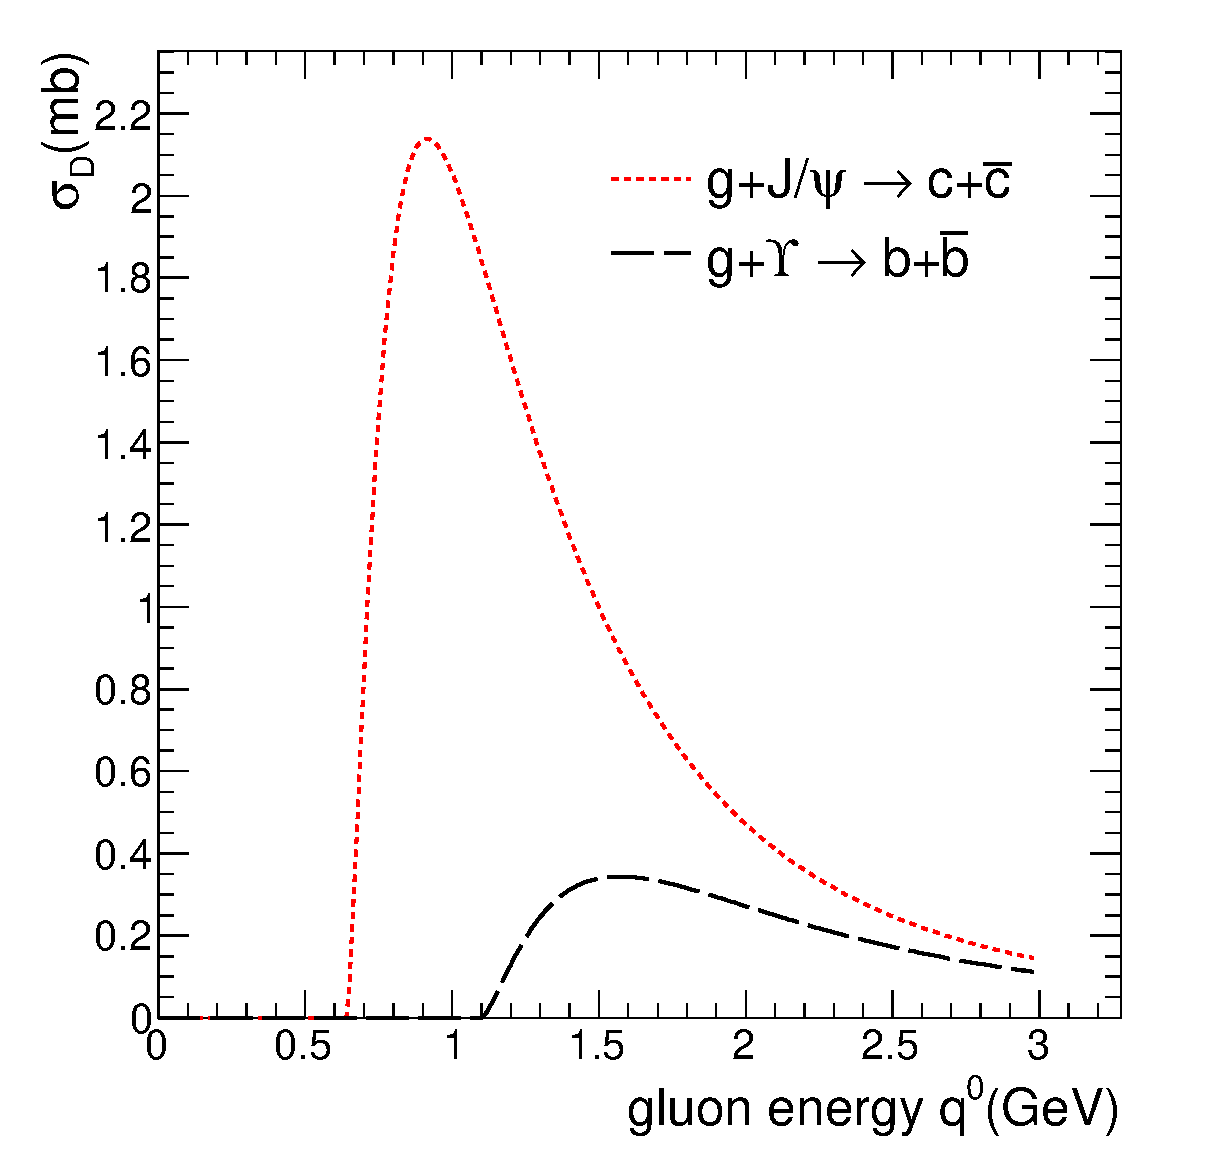
\includegraphics[width=0.60\textwidth]{Figures/Fig2_SigmaDq0.eps}
\caption{Gluon dissociation cross-section of quarkonia as a function of gluon energy ($q^{0}$) in
quarkonia rest frame.}
\label{fig:SigmaDQ0}
\end{figure}

\begin{figure}
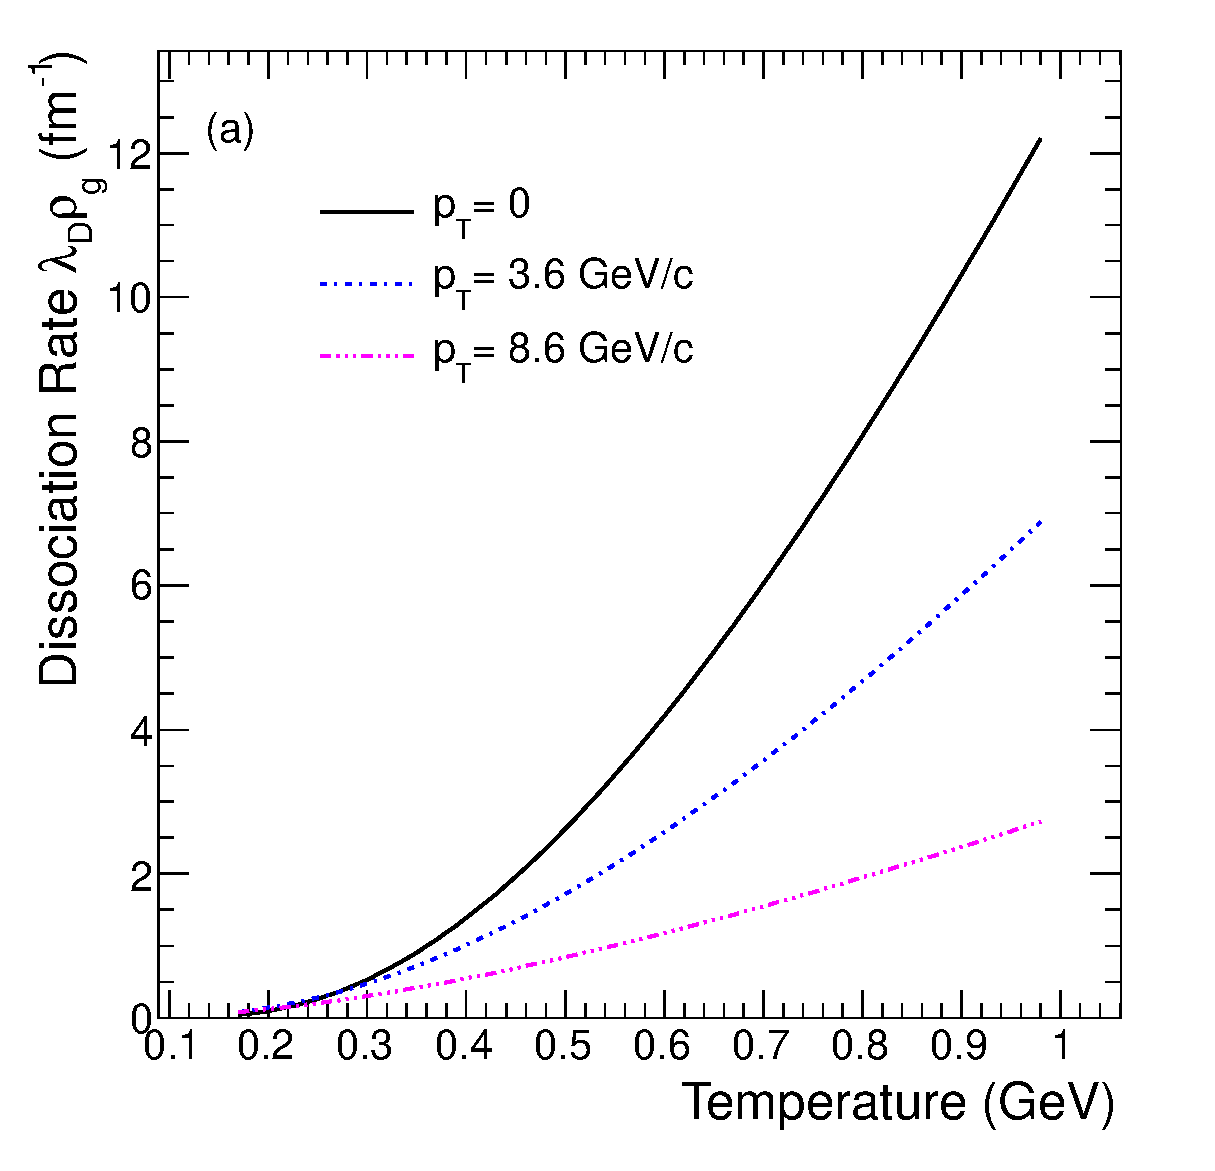
\includegraphics[width=0.49\textwidth]{Figures/Fig3a_DRateVsT.eps}
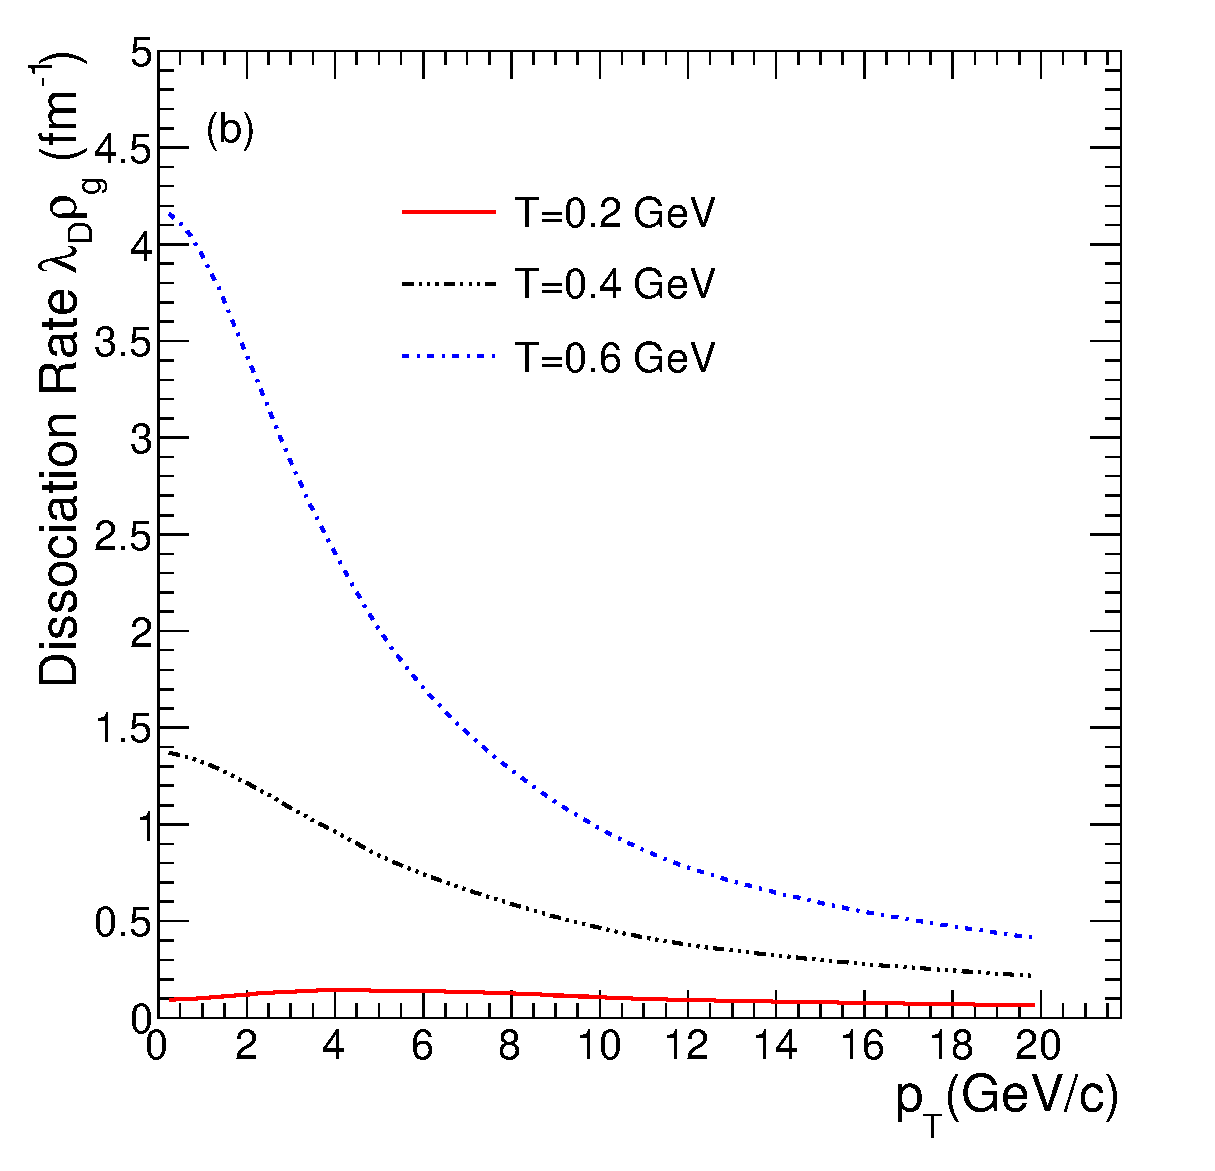
\includegraphics[width=0.49\textwidth]{Figures/Fig3b_DRateVsPt.eps}
\caption{(Color online) Gluon dissociation rate of $\Jpsi$ as a function of a) temperature and  b) transverse momentum.}
\label{fig:DRateVsTempAndPt}
\end{figure}


%
%and $q^0$ the gluon energy in the $J/ \psi$ rest frame is related to centre of mass 
%energy of $\Jpsi$-gluon system as
%\begin{eqnarray}
% q^{0} = \frac{s-M_{\Jpsi}^{2}}{2\,M_{\Jpsi}},
%\end{eqnarray}

%%%%%%%%%%%%%%%%%%%%%%%%%%%%%%%%%%%%%%%%%%%%%%%%%%%%%%%%%%%%%%%%%%%%
%%%%%%%%%%%%%%%%%%%%%%%%%%%%%%%%%%%%%%%%%%%%%%%%%%%%%%%%%%%%%%%%%%
%`If we consider that the $J/ \psi$ moves in the transverse direction with a four-velocity
%$u=(M_T, \vec{P_T}, 0)/M_{\Jpsi}$, where $M_T=\sqrt{p_T^2+M^2_{J/ \psi}}$ is defined as the $\Jpsi$'s
%transverse mass. 
%A gluon with a four-momentum $k=(k^0,\vec{k})$
%in the rest frame of the parton gas has an energy $q^0=k\cdot u$
%in the rest frame of the $\Jpsi$ given by
%\begin{eqnarray}
% q^{0} &= &\frac{k^{0}\,m_{T} + \vec{k} \cdot \vec{p_{T}}}{M_{\Jpsi}}, \nonumber \\
%       &= &\frac{s-M_{\Jpsi}^{2}}{2\,M_{\Jpsi}},
%\end{eqnarray}
%The dissociation rate is given by 
%\begin{eqnarray}
%\lambda_D = \langle v_{\rm rel} \sigma_{D} (k \cdot u)\rangle_k &= &\frac{\int d^3k v_{\rm rel} \sigma_{D} (k \cdot u) f(k^0,T)}{\int d^3k f(k^0,T)},
% \label{eq5}
%\end{eqnarray}
%where the gluon distribution in the rest frame of the parton gas is
%\begin{equation}
%  f(k^0,T)=\frac{\lambda_g(=16)}{e^{k^0/T}-1} \label{eq6}.
%\end{equation}
%The relative velocity $v_{\rm rel}$ between the $\Jpsi$ and a gluon is
%\begin{eqnarray}
% v_{\rm rel}  =  \frac{P_{\Jpsi}\cdot k}{k^0M_T} \,\,
%              =  1-\frac{\vec{k}\cdot\vec{P}_T}{k^0M_T} \,\,
%              =  {s- M_{\Jpsi} \over 2E_1E_2}  
%\label{eq7}
%\end{eqnarray}
%Changing the variable to the gluon momentum, $q=(q^0,\vec{q})$, in
%the rest frame of the $\Jpsi$, and writing $\rho_g = \int d^3k f(k^0,T)$, 
%the Eq.~(\ref{eq5}) can be rewritten as
%\begin{eqnarray}
%\lambda_D \rho_g  =  \int d^3q \frac{M_{\Jpsi}}{m_T}\sigma_{D}(q^0) f(k^0,T).
%\label{eq8}
%\end{eqnarray}
%Using $ k^0=(q^0M_T+\vec{q}\cdot\vec{P}_T)/M_{\Jpsi}$ in Eq.~\ref{eq8} and solving
%\begin{eqnarray} 
%\lambda_D\,\rho_g &= &\frac{M_{\Jpsi}}{m_T} \int d^3q \, \sigma_{D}(q^0) \frac{\lambda_{g}} {  e^{ \frac{q^0m_{T}}{M_{\Jpsi}T}} e^{ \frac{ \vec{q}\cdot \vec{p_{T} } }{ M_{\Jpsi}T }  } -1}  \nonumber \\
%%&= &\frac{\lambda_{g}}{2\pi^3} \frac{M_{\Jpsi}}{m_T} \int d^3q \, \sigma_{D}(q^0)   \sum_{n=1}^{\infty}  e^{ \frac{-n\,q^0 m_{T}}{M_{\Jpsi}T}} e^{  \frac{-n\,\vec{q}\cdot \vec{p_{T}}}{M_{\Jpsi}T}}  \nonumber \\
%%&= &\frac{\lambda_{g}}{2\pi^3} \frac{M_{\Jpsi}}{m_T}  \sum_{n=1}^{\infty} 2\pi  \int (q^0)^2 dq^0 \, \sigma_{D}(q^0)\,e^{ \frac{-n\,q^0m_{T}}{M_{\Jpsi}T}}  \int_{1}^{-1} e^{  \frac{-n\,q^0\,p_{T} cos\theta}{M_{\Jpsi}T}} d(cos\theta) \nonumber \\
%%&= &\frac{\lambda_{g}}{2\pi^3} \frac{M_{\Jpsi}}{m_T} \sum_{n=1}^{\infty} 2\pi  \int (q^0)^2 dq^0 \, \sigma_{D}(q^0)\,e^{ \frac{-n\,q^0 m_{T}}{M_{\Jpsi}T}} 
%%    \left[ e^{-\frac{nq^0 p_T}{M_{\Jpsi}T}} - e^{\frac{nq^0 p_T}{M_{\Jpsi}T}} \right]\,\frac{M_{\Jpsi}T}{nq^0 p_T}  \nonumber \\
%&= &\frac{\lambda_{g}}{2\pi^3} \frac{M_{\Jpsi}^2}{m_T} 2\pi \sum_{n=1}^{\infty} \frac{T}{n} \int_{\epsilon_0}^{\infty} q^0 dq^0 \, \sigma_{D}(q^0)  
%     \,e^{ \frac{-n\,q^0 m_{T}}{M_{\Jpsi}T}} 
%     \frac{1}{p_T} \left[e^{\frac{n q^0 p_T}{M_{\Jpsi}T}} - e^{- \frac{n q^0 p_T}{M_{\Jpsi}T}}\right] \\ \nonumber
%\label{dissrate}
%\end{eqnarray}

%%%%%%%%%%%%%%%%%%%%%%%%%%%%%%%%%%%%%%%%%%%%%%%%%%%%%%%%%%%%%%%%%%%%
%%%%%%%%%%%%%%%%%%%%%%%%%%%%%%%%%%%%%%%%%%%%%%%%%%%%%%%%%%%%%%%%%%%%
% The special case of Eq.~(\ref{dissrate}) for J/$\psi \,p_T = 0$ is
%\begin{eqnarray} 
%  \frac{1}{p_T} \left[e^{\frac{n q^0 p_T}{M_{\Jpsi}T}} - e^{- \frac{n q^0 p_T}{M_{\Jpsi}T}}\right] = {2nq^0\over M_{\Jpsi}T}.
%\label{case}
%\end{eqnarray}
%Using this we get 
%\begin{eqnarray} 
% \lambda_D\,\rho_g &= &  4\pi \int (q^0)^2\,dq^0 \, \sigma_{D}(q^0) \frac{\lambda_{g}} {e^{\frac{q^0}{T}} -1}
%\end{eqnarray}

%%%%%%%%%%%%%%%%%%%%%%%%%%%%%%%%%%%%%%%%%%%%%%%%%%%%%%%%%%%%%%%%%%%%%%%%%%%%%%%%%%%%
\subsection{Formation Rate}
  We can calculate formation cross section from dissociation cross section using detailed balance 
relation \cite{Thews:2000rj,Thews:2005vj} as
\begin{equation}
\sigma_{F} = \frac{48}{30}\,\sigma_{D}(q^0)\frac{(s-M_{\Jpsi})^{2}}{s(s-4m_{c}^{2})}.
\end{equation}
The formation rate can be written as
\begin{equation}
\lambda_{F} = \langle \sigma_{F} \,\, v_{\rm rel}(s) \rangle = \frac{\int \sigma_{F}(s)\, v_{\rm rel}\,f_{c}(p_1)\, f_{\bar{c}} (p_2) \,d^{3}p_1 \,d^{3}p_2 \, \delta^{3}(\vec{p}-(\vec{p_1}+\vec{p_2}))} 
       {\int \,f_{c}(p_1)\,d^{3}p_1 \,\, \int f_{\bar{c}} (p_2)\,d^{3}p_2}.
\end{equation}
Here $f_{c/\bar{c}}(p)$ are taken as thermal distribution function of  $c/\bar{c}$.
$v_{\rm rel}$ is relative velocity between c $\bar{c}$ quark pair and is given by
\begin{eqnarray}
v_{\rm rel} &=& {\sqrt{(p_{1}.p_{2})^{2} - m_{c}^{4} } \over E_{1} \, E_{2}} \nonumber \\
            &=& \frac{\sqrt{s(s-4m_{c}^{2})}}{2E_1E_2}.
\end{eqnarray}
 Here $p_1 = (E_1,\vec{p_{1}})$, $p_{2} = (E_{2},\vec{p_{2}})$ are four momenta of charm and anti-charm 
quarks, respectively. The centre of mass energy square of c$\bar{c}$ system is 
 $s =  2\,m_c^{2} + 2 E_1E_2 - 2 |\vec{p_1}||\vec{p_2}|cos\theta$.

Figure \ref{fig:ForRateVsTempAndPt} shows variation of formation rate as a funcion of medium temperature
and transverse momentum. The $\Jpsi$ generated from recombination of uncorrelated heavy quark pairs will have 
softer $p_{T}$ distributions than that of $\Jpsi$ coming from initial hard scattering and thus 
effect of recombination will be important only at low $p_T$.

\begin{figure}
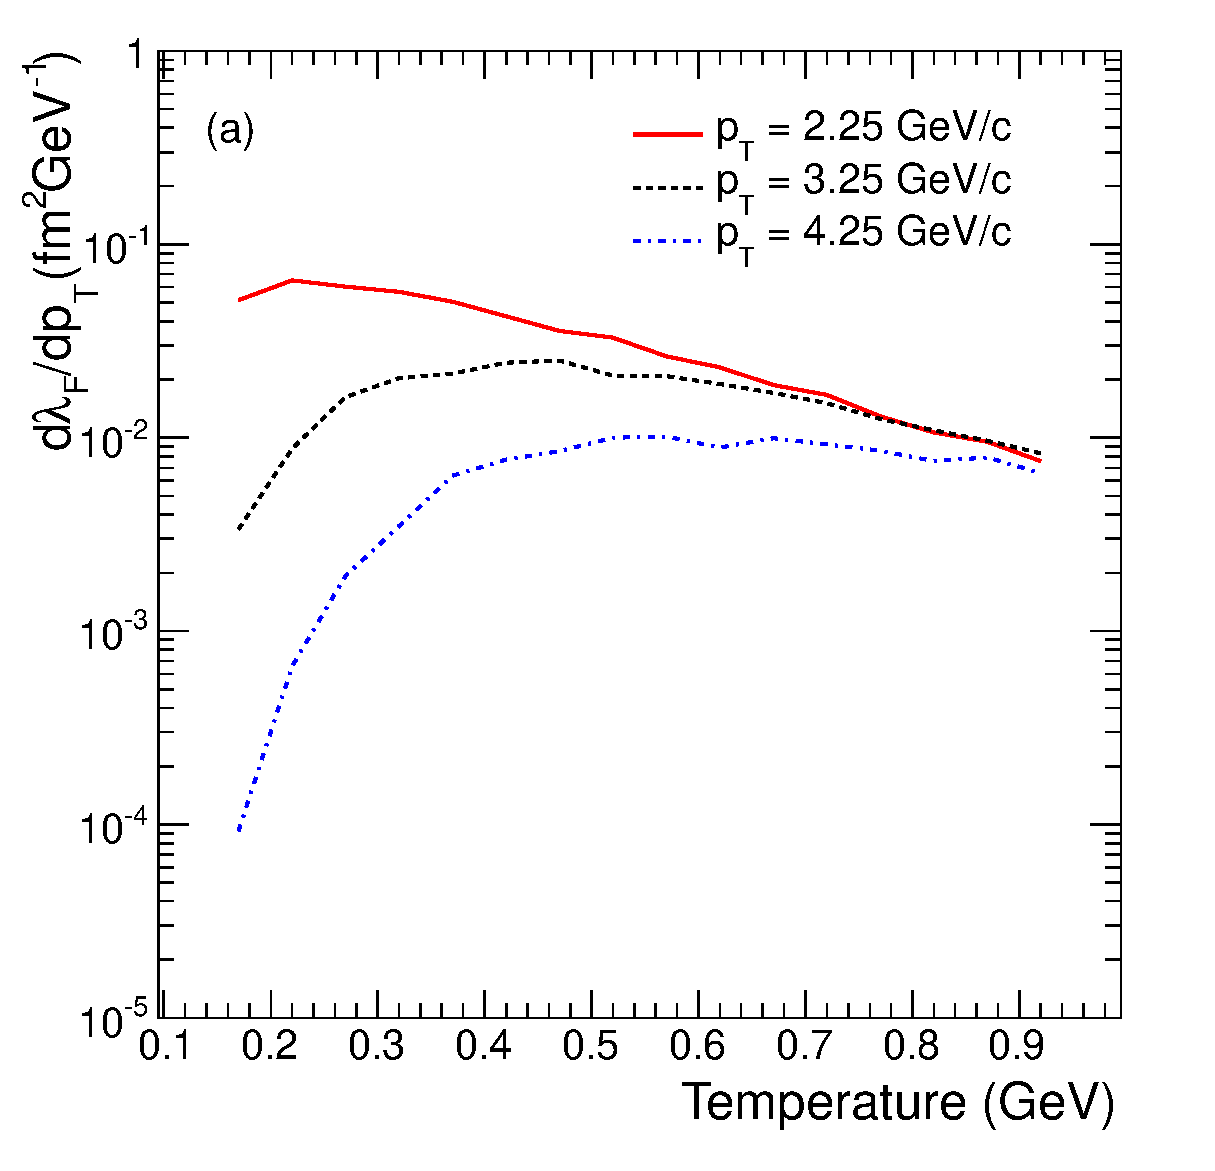
\includegraphics[width=0.49\textwidth]{Figures/Fig4a_FRateVsT.eps}
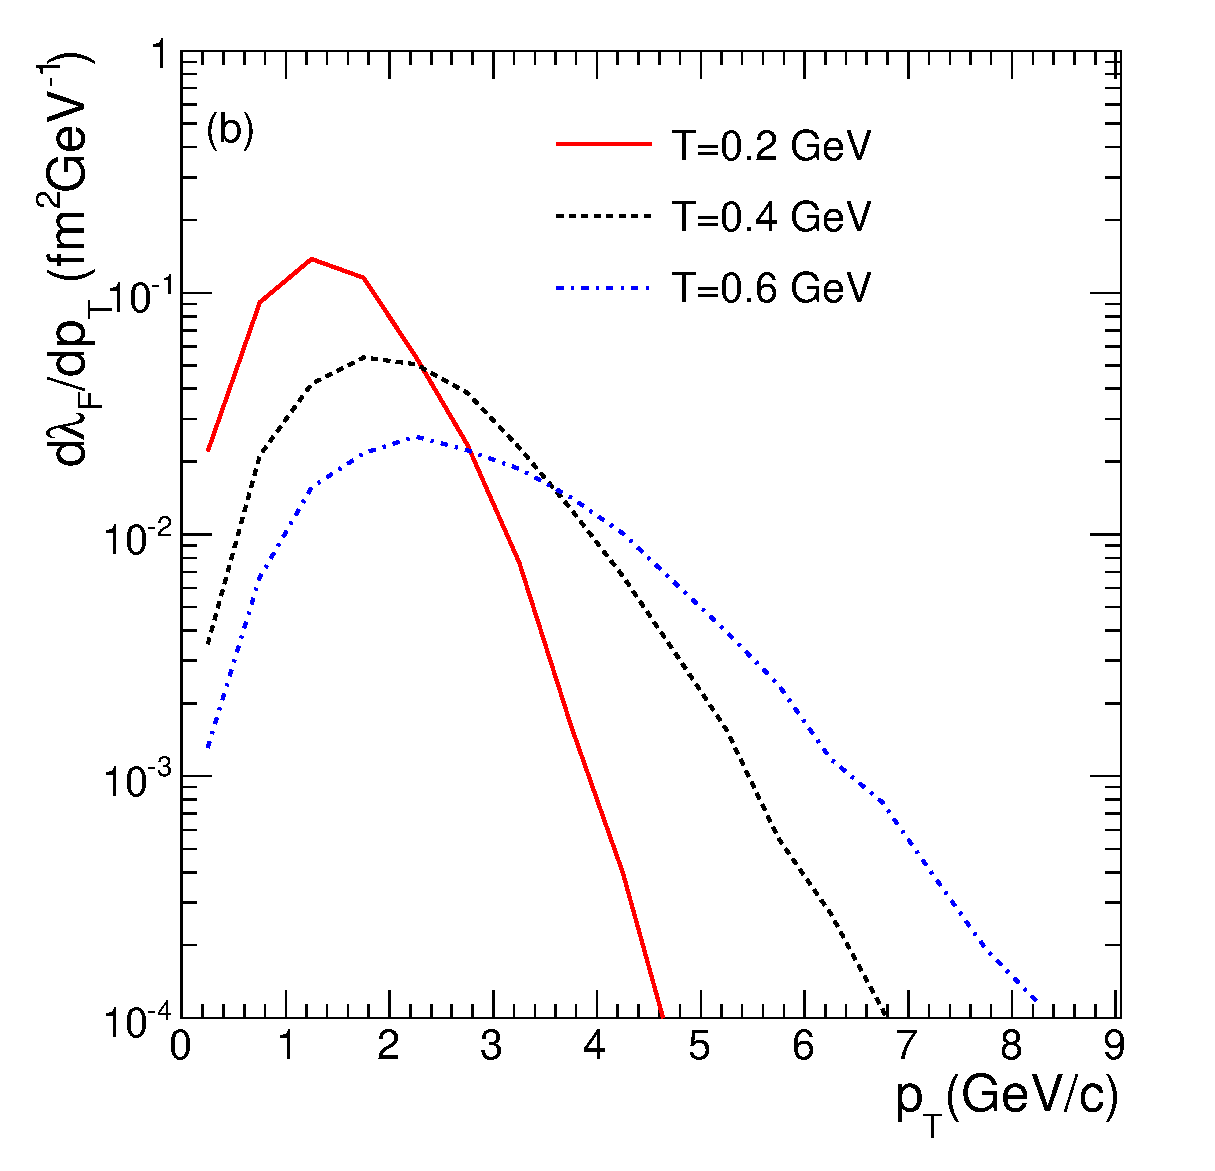
\includegraphics[width=0.49\textwidth]{Figures/Fig4b_FRateVsPt.eps}
\caption{(Color online) Formation rate as a function of (a) temperature and (b) transverse momentum.}
\label{fig:ForRateVsTempAndPt}
\end{figure}

The formation and dissociation rates are shown for $\Jpsi$, we use same formalism to calculate
these rates for $\Upsilon$ also.


\begin{figure}
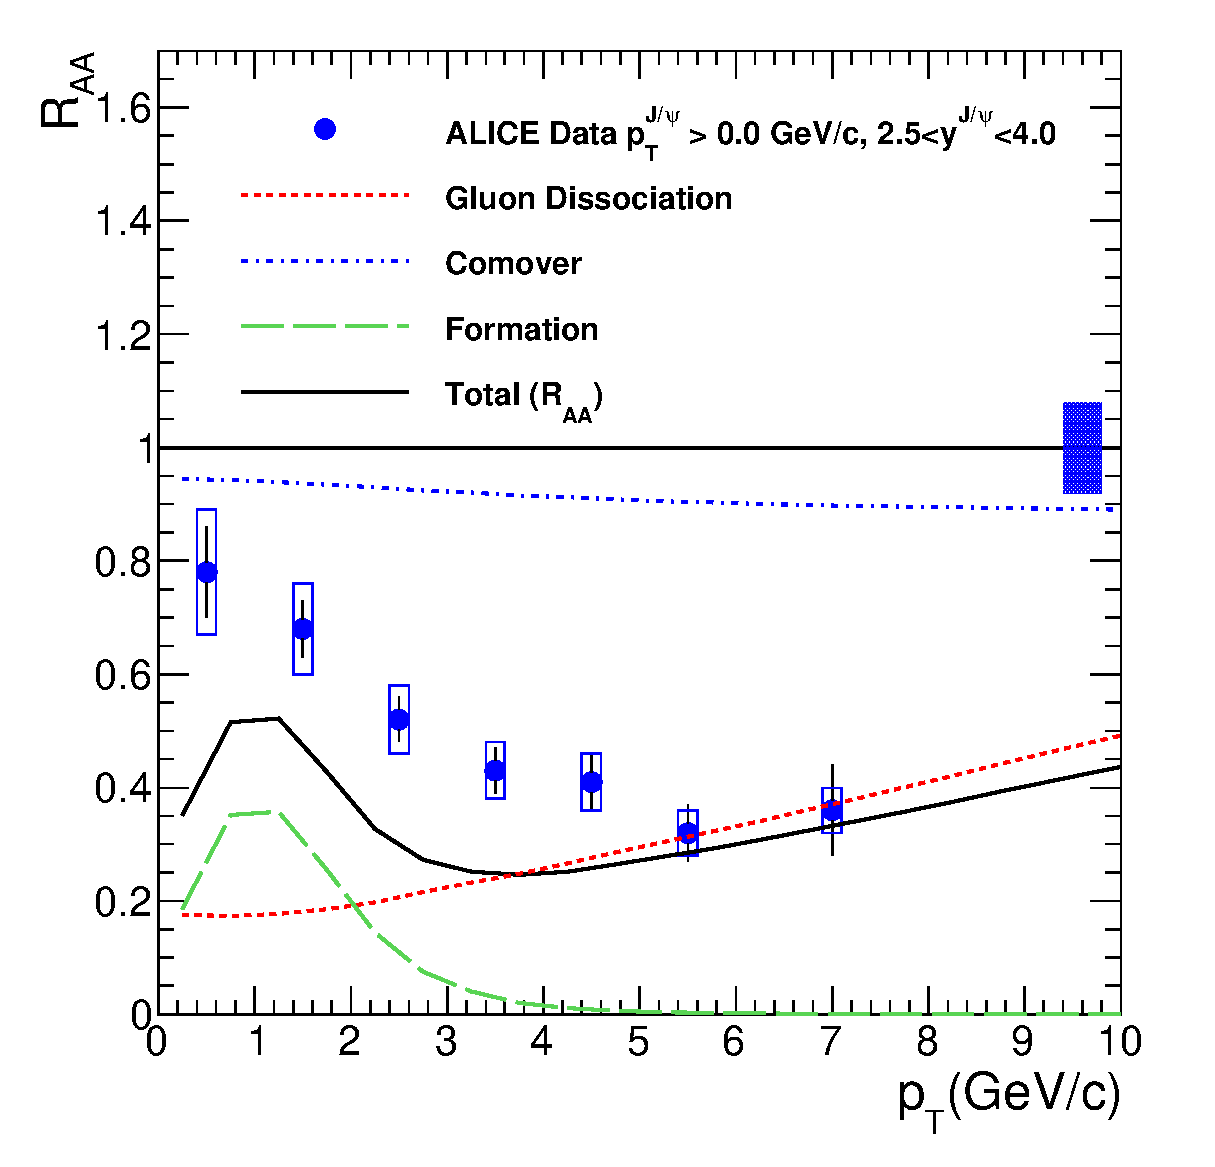
\includegraphics[width=0.49\textwidth]{Figures/Fig5a_ALICE_RAAPt.eps}
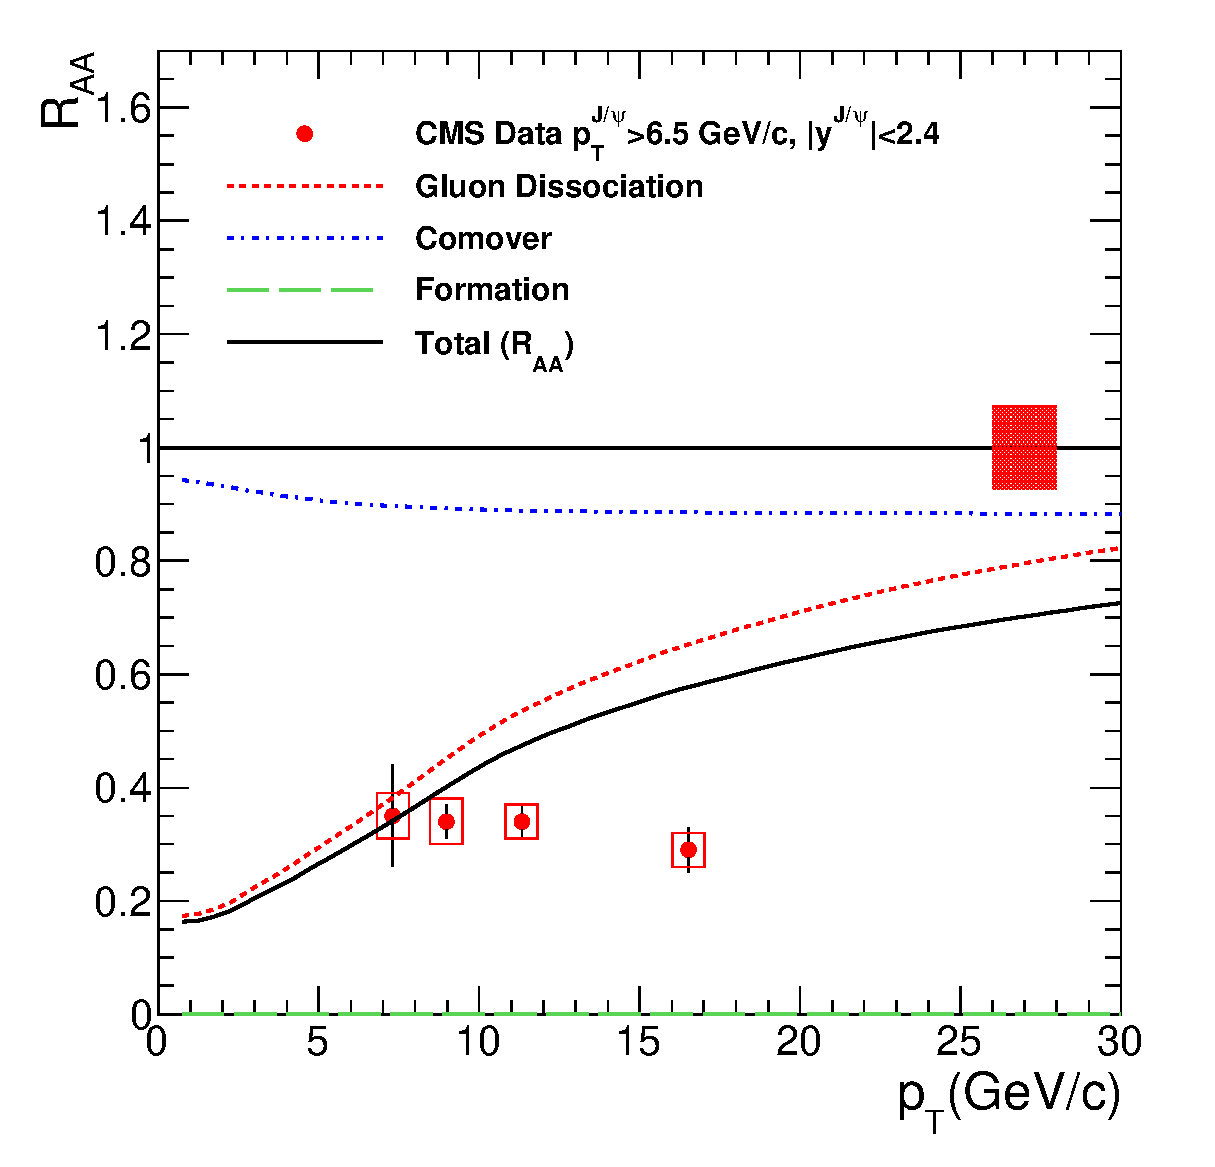
\includegraphics[width=0.49\textwidth]{Figures/Fig5b_CMS_RAAPt.eps}
\caption{(Color online) Calculated nuclear modification factor (R$_{AA}$) as a function of $\Jpsi$ transverse momentum. Calculations are
compared with ALICE and CMS measurements.}
\label{fig:JPsiRaaVsPt}
\end{figure}


%%%%%%%%%%%%%%%%%%%%%%%%%%%%%%%%%%%%%%%%%%%%%%%%%%%%%%%%%%%%%%%%%%%%%%%%%%%%%%%%%%%%%%
%\section{Formation of quarkonia  by statistical hadronization model}\label{SHM}
% The heavy quark production at LHC is substantial which may lead to incoherent 
%recombination of uncorrelated pairs of heavy quarks and anti quarks which result 
%from multiple pair production. In statistical approach \cite{MUNZI} the number of 
%$\Jpsi$ regenrated is given by 
%\begin{eqnarray}
%N_{\Jpsi}  &= &4 {n_{ch} n_{\Jpsi} \over n_{\rm open}^2}  {N_{c\bar c}^2 \over N_{ch} }\\
%          &= &\frac{N_{c\overline{c}}^{2}}{V}\frac{4n_{\Jpsi}}{n_{open}^{2}}.
%\end{eqnarray}
%where $n_i$'s are the thermal densities, $N_{c\bar c}$ is the number of charm pairs produced 
%and $N_{ch}$ is the number of total charged particle produced. 
%The freeze out parameters are $T=170$ MeV and $\mu_B = 0$. For
%$dN_{ch}/dy = 1600$ \cite{MULT} and $dN_{c \bar c} /dy = 14.0$, we obtain $dN_{\Jpsi} /dy = 0.0092$.


\begin{figure}
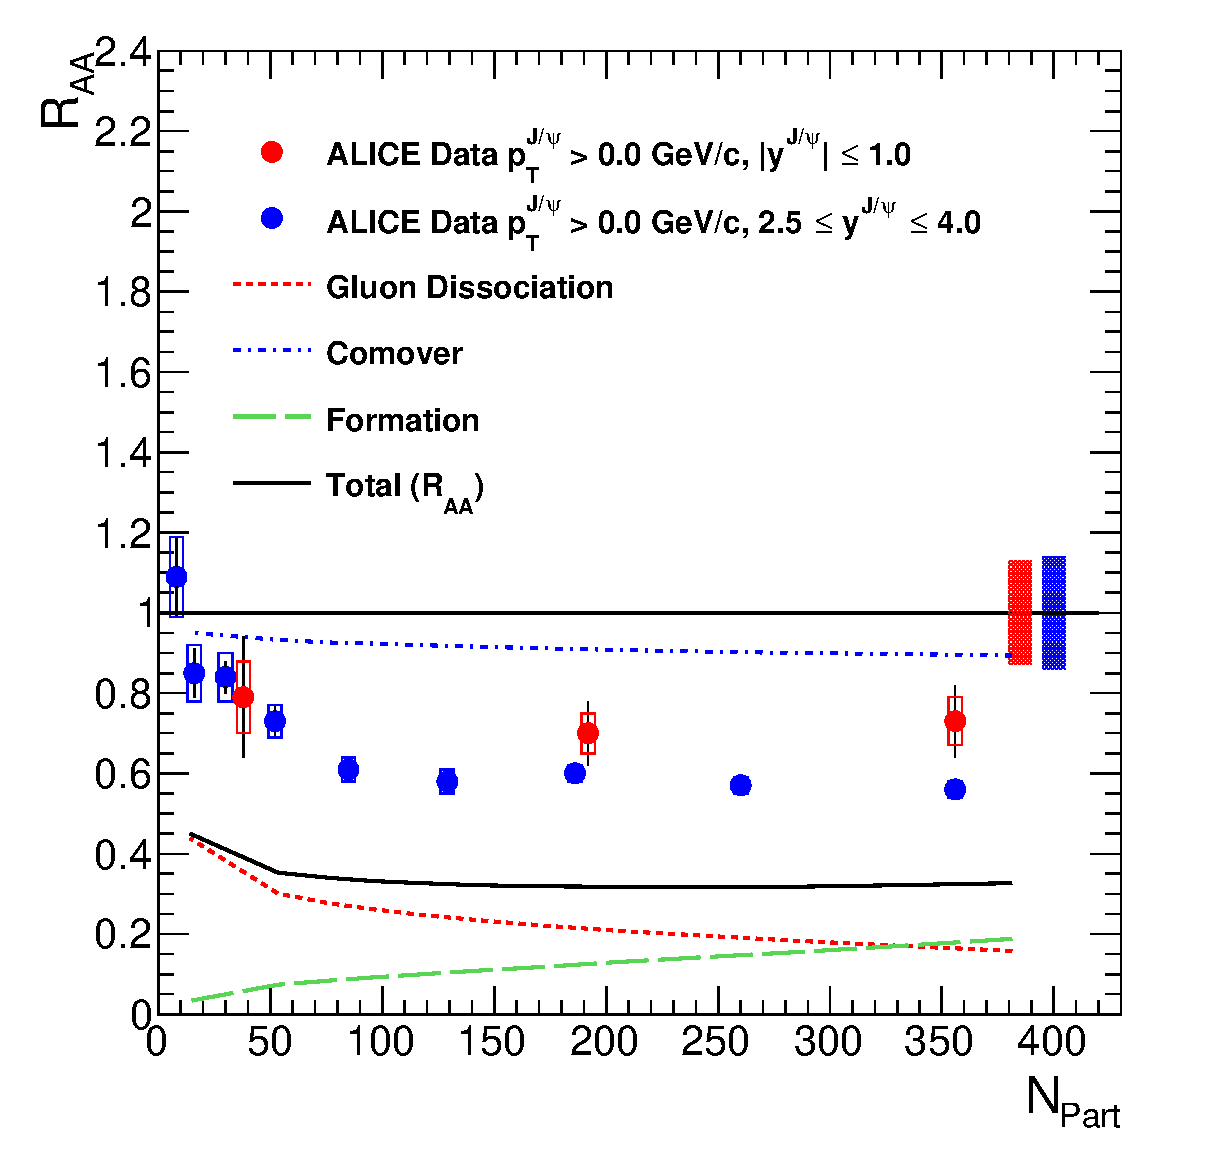
\includegraphics[width=0.49\textwidth]{Figures/Fig6a_ALICE_RAANPart.eps}
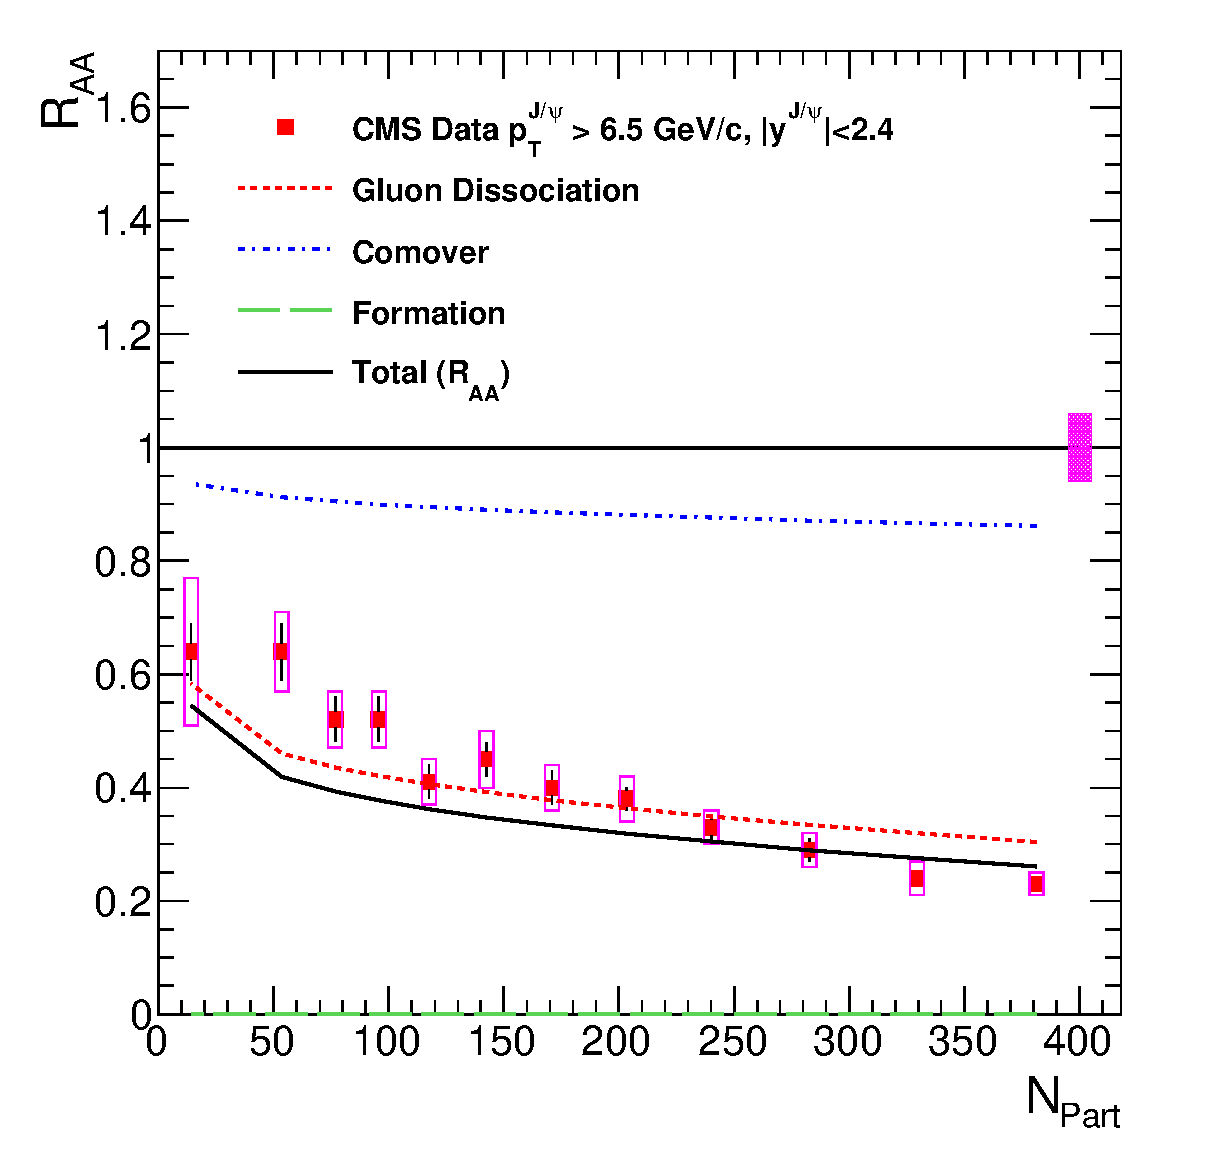
\includegraphics[width=0.49\textwidth]{Figures/Fig6b_CMS_RAANPart.eps}
%\caption{(Color online) Calculated nuclear modification factor (R$_{AA}$) compared with ALICE and CMS measurements at LHC. No regeneration is 
%considered for high p$_{T}$ CMS data. We assume similar cold nuclear matter effects for both ALICE and CMS rapidity ranges.}
\caption{(Color online) Calculated nuclear modification factor (R$_{AA}$) compared with ALICE and CMS measurements at LHC. No regeneration is 
considered for high p$_{T}$ CMS data. We assume similar cold nuclear matter effects for both ALICE and CMS rapidity ranges.}
\label{fig:JPsiRaa}
\end{figure}


\begin{figure}
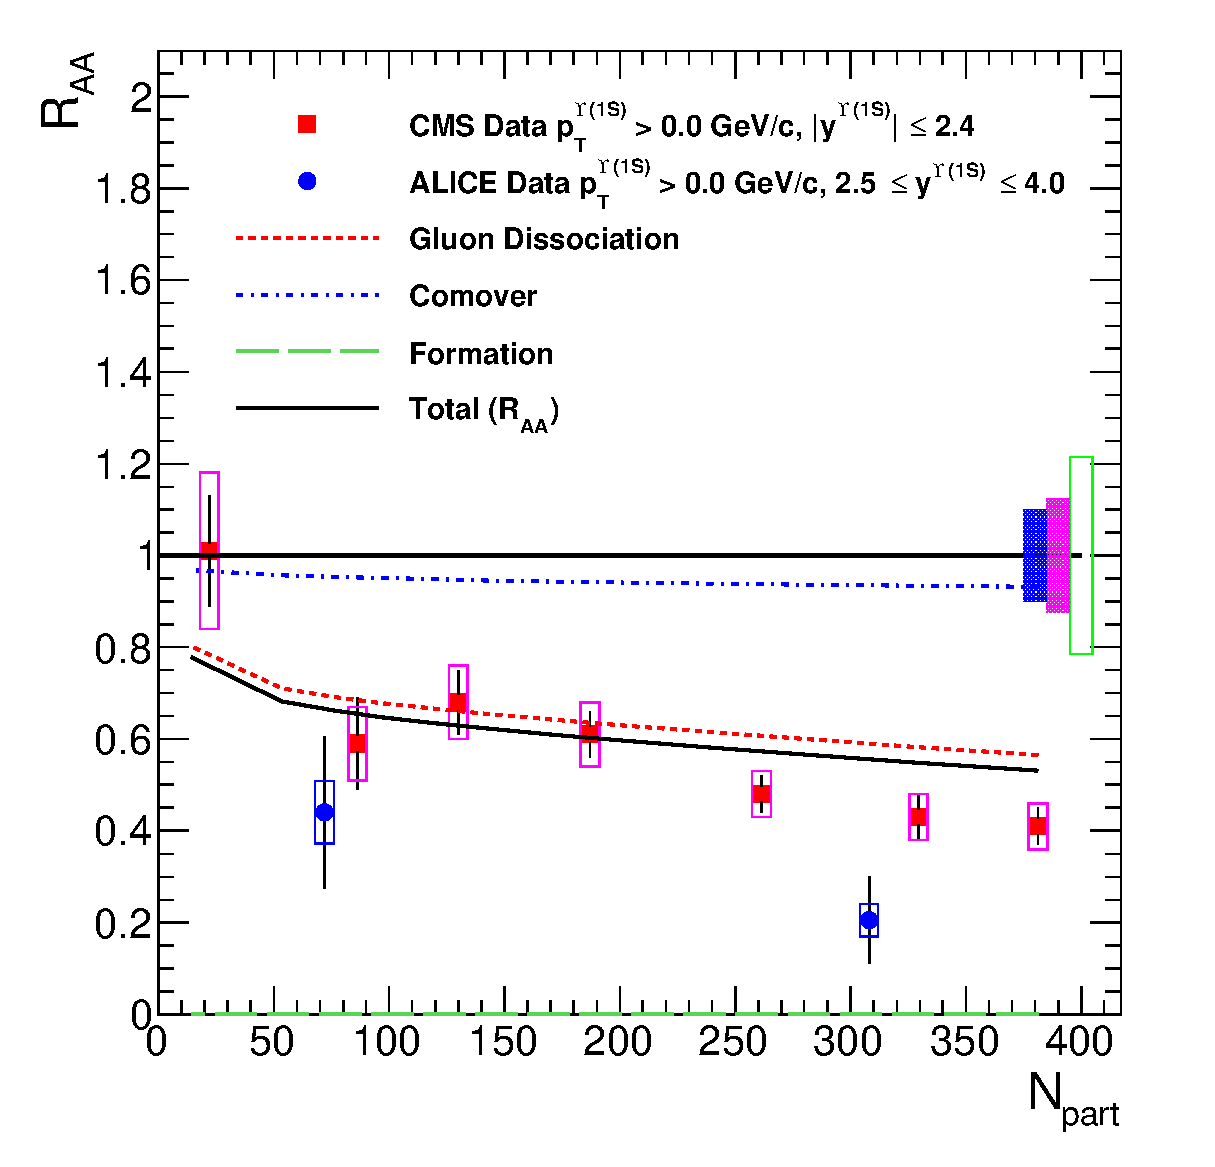
\includegraphics[width=0.49\textwidth]{Figures/Fig7a_CMS_Y1SRAANPart.eps}
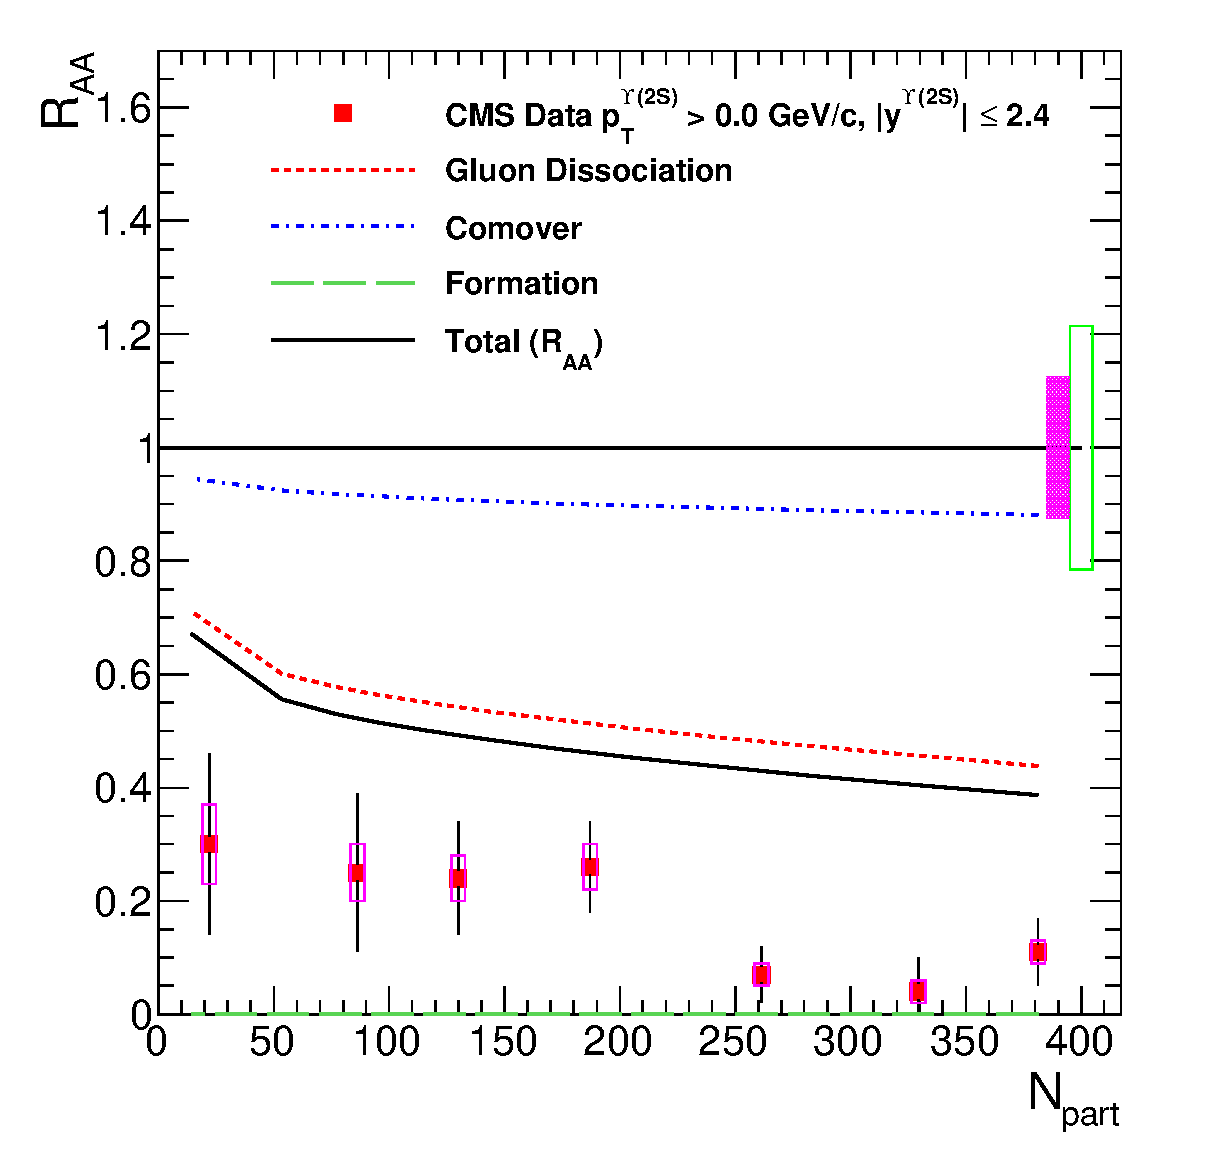
\includegraphics[width=0.49\textwidth]{Figures/Fig7b_CMS_Y2SRAANPart.eps}
%\caption{(Color online) Calculated nuclear modification factor (R$_{AA}$) compared with CMS $\Upsilon$(1S) and $\Upsilon$(2S) measurements.
%We assume small cold nuclear matter suppression than J$\psi$ and no regeneration due to small production cross section of beauty quark as shown in Table~\ref{NLOcros}.}
\caption{(Color online) Calculated nuclear modification factor (R$_{AA}$) compared with CMS $\Upsilon$(1S) and $\Upsilon$(2S) measurements.
We assume small cold nuclear matter suppression than J$\psi$ and no regeneration due to small production cross section of beauty quark as shown in Table~\ref{NLOcros}.}
\label{fig:UpsilonRaa}
\end{figure}

%%%%%%%%%%%%%%%%%%%%%%%%%%%%%%%%%%%%%%%%%%%%%%%%%%%%%%%%%%%%%%%%%%%%%%%%%%%%%%%%%%%%%%%%
\section{Cold matter effects}
%The quarkonia can be suppressed due to cold matter effects such as shadowing and due to hadronic
%and comover interaction. For simplicity we approximate the combination of all CNM effects 
%by a suppression factor \cite{Rapp1,Rapp2},
%\begin{equation}
%  S_{Nucl}=\exp[-\rho_{N}\sigma_{abs}L(b)]
%  \label{CNMF}
%\end{equation}
%with an effective nuclear absorption cross section, $\sigma_{abs}$.
%We take absorption cross section, $\sigma_{abs}$ = 1.5 mb (1.5 mb) for
%$\Jpsi$($\Upsilon$). The other parameters in Eq. \ref{CNMF} are the nuclear density,
%$\rho_N$=0.14 fm$^{-3}$, and the impact-parameter dependent path length, L(b), evaluated 
%with a Glauber model \cite{GM_PShukla} for the nuclear overlap.
  The suppression of quarkonia by comoving pions can be calculated by folding the $\Jpsi$-pion
dissociation cross section $\sigma_{\rm I}$ over thermal pion distributions \cite{Vogt:1988fj}. 
It is expected  that at LHC energies cross-section of comover suppression will be small \cite{Lourenco:2008sk}.
We take 1 mb cross-section for both $\Jpsi$ and $\Upsilon$ states.  
The dissociation rate $\lambda_{D_{\pi}}$  can be written as
\begin{eqnarray}
\lambda_{D_{\pi}} \, \rho_{\pi} & = & \frac{g_\pi}{(2\pi)^{3}} \int d^{3}p f_{\pi}(p) v_{\rm rel} \sigma_{I}\\ \nonumber
                   & = &\frac{g_\pi}{(2\pi)^{3}} \int  2\pi p^{2} dp f_{\pi}(p) \int \sigma_{\rm I} v_{\rm rel}(s) \Theta(s-4m_{D}^{2}) d(cos\theta) \\\nonumber
\end{eqnarray}
where $f_{\pi}(p,T)$ is taken as the thermal pion distribution and the  pion density $\rho_{\pi}$ is given by 
\begin{eqnarray}
\rho_\pi =\frac{g_\pi}{(2\pi)^{3}} \int d^3p \, f_{\pi}(p) 
\end{eqnarray}

The survival probability from pion collisions at freeze-out time $\tau_f$ is written as
\begin{equation}
S(p_T) = \exp \left( {-\int_{\tau_0}^{\tau_f} (1-f(\tau)) \lambda_{D_{\pi}}(T,p_T)\,\rho_{\pi}(T)\,d\tau} \right).
\end{equation}
The temperature $T(\tau)$ and the hadronic fraction (1-$f(\tau)$) 
evolve from phase transition time to freeze-out time.


\section{Results and discussion}
  Figure~\ref{fig:JPsiRaaVsPt} shows our calculations of 
nuclear modification factor ($R_{AA}$) of $\Jpsi$ as a function of transverse momentum 
along with the measurements by  ALICE \cite{Abelev:2013ila} and CMS \cite{Mironov:2013jaa} experiments.
 Our model with gluon dissociation, $\Jpsi$ regeneration and comover suppression describes the 
ALICE data very well in (a). However only gluon dissociation is not enough to explain the $\Jpsi$ 
high $p_{T}$ data measured by CMS experiment in (b). 
  We consider the contributions of recombined $\Jpsi$ only for low $p_{T}$ 
measurements made by ALICE. We can notice from figure~\ref{fig:JPsiRaaVsPt} (a) 
that regenerated $\Jpsi$ have very soft $p_{T}$ distribution and
contribution after 4-5 GeV/c is negligible 
Figure~\ref{fig:JPsiRaa} (a) shows comparison of our calculations with $\Jpsi$ 
nuclear modification factor as a function of event centrality measured by ALICE \cite{Abelev:2013ila}
experiment in forward and central rapidities. Our calculations predict
stronger suppression than observed in ALICE measurement.
%the data very well in both mid and forward rapidity region.
Figure~\ref{fig:JPsiRaa} (b) shows $R_{AA}$ of $ \Jpsi$ with $p_{T}\,\geq$ 6.5 GeV/c, measured 
by CMS experiment \cite{Mironov:2013jaa}. It shows large suppression with strong centrality dependence. Our
calculations are in good agreement with measured data.   
Figure~\ref{fig:UpsilonRaa} (a) shows centrality dependence of $\Upsilon(1S)$ nuclear modification factor
measured in mid rapidity by CMS experiment\cite{Chatrchyan:2012lxa} and in forward rapidity by ALICE experiment 
\cite{Abelev:2014nua}. Our calculations matches very well with measurement except in most central collisions.
Figure~\ref{fig:UpsilonRaa} (b) shows centrality dependence of $\Upsilon(2S)$ nuclear modification factor
measured in mid rapidity by CMS experiment. Only gluon dissociation is not enough to explain the strong 
suppression observed in measurement. There may be higher oreder effects like lowering of binding energy 
of bound states at high tempreture, which we do not consider in this calculation. As production cross section of 
bottom quark is small even at LHC energies, we do not consider effect of recombination for $\Upsilon$ calculations.
%%%%%%%%%%%%%%%%%%%%%%%%%%%%%%%%%%%%%%%%%%%%%%%%%%%%%%%%%%%%%%%%%%%%%%%%%%%%%%%%%%%%%%%
\section{Summary}
 We have carried out detailed calculations of $\Jpsi$ and $\Upsilon$ 
modifications in PbPb collisions at LHC.
  The $\Jpsi$ suppression is estimated using process of gluon dissociation in medium. 
The rate of regeneration has been obtained using principle of detailed balance.
  The dissociation and formation rates have been studied a function of medium temperature
and transverse momentum of particles.
  The nuclear modification factor as a function of centrality and transverse momentum has been calculated  
and compared to $\Jpsi$ and $\Upsilon$ nuclear modification factors measured in PbPb collisions 
at $\sqrt s_{NN}$ =  2.76 TeV.


\noindent
\begin{thebibliography}{100}
\medskip
%\bibitem{SATZ} T. Matsui and H. Satz, Phys. Lett. B{\bf 178}, 416 (1986).
%\cite{Matsui:1986dk}
\bibitem{Matsui:1986dk} 
 T.~Matsui and H.~Satz,
 ``$J/\psi$ Suppression by Quark-Gluon Plasma Formation'',
 Phys.\ Lett.\ B {\bf 178}, 416 (1986).
 %%CITATION = PHLTA,B178,416;%%
 %1936 citations counted in INSPIRE as of 18 Jun 2014

%\bibitem{Schukraft} J. Schukraft, arXiv:1311.1429 [hep-ex].
%\cite{Schukraft:2013wba}
\bibitem{Schukraft:2013wba} 
  J.~Schukraft,
  ``Heavy Ion Physics at the LHC: What's new ? What's next ?'',
  arXiv:1311.1429 [hep-ex].
  %%CITATION = ARXIV:1311.1429;%%
  %4 citations counted in INSPIRE as of 18 Jun 2014

%\bibitem{Kluberg:2009wc} L.~Kluberg and H.~Satz, arXiv:0901.3831 [hep-ph].
%\cite{Kluberg:2009wc}
\bibitem{Kluberg:2009wc} 
  L.~Kluberg and H.~Satz,
  ``Color Deconfinement and Charmonium Production in Nuclear Collisions,''
  arXiv:0901.3831 [hep-ph].
  %%CITATION = ARXIV:0901.3831;%%
  %50 citations counted in INSPIRE as of 18 Jun 2014

%\bibitem{Brambilla:2010cs}  N.~Brambilla, S.~Eidelman, B.~K.~Heltsley, R.~Vogt, G.~T.~Bodwin, 
%  E.~Eichten, A.~D.~Frawley and A.~B.~Meyer {\it et al.},  Eur.\ Phys.\ J.\ C{\bf 71}, 1534 (2011),
% arXiv:1010.5827 [hep-ph].
%\cite{Brambilla:2010cs}
\bibitem{Brambilla:2010cs} 
  N.~Brambilla, S.~Eidelman, B.~K.~Heltsley, R.~Vogt, G.~T.~Bodwin, E.~Eichten, A.~D.~Frawley and A.~B.~Meyer {\it et al.},
  ``Heavy quarkonium: progress, puzzles, and opportunities,''
  Eur.\ Phys.\ J.\ C {\bf 71}, 1534 (2011)
  [arXiv:1010.5827 [hep-ph]].
  %%CITATION = ARXIV:1010.5827;%%
  %577 citations counted in INSPIRE as of 18 Jun 2014


%\bibitem{PHENIXJPsi} A. Adare {\it et al.} (PHENIX Collaboration) Phys. Rev. C{\bf 84}, 054912 (2011), arXiv: 1103.6269.
%\cite{Adare:2011yf}
\bibitem{Adare:2011yf} 
  A.~Adare {\it et al.}  [PHENIX Collaboration],
  ``$J/\psi$ suppression at forward rapidity in Au+Au collisions at $\sqrt{s_{NN}}=200$ GeV,''
  Phys.\ Rev.\ C {\bf 84}, 054912 (2011)
  [arXiv:1103.6269 [nucl-ex]].
  %%CITATION = ARXIV:1103.6269;%%
  %94 citations counted in INSPIRE as of 18 Jun 2014

%\bibitem{Andronic_SH1} A. Andronic, P. Braun-Munzinger, K. Redlich, J. Stachel, Phys. Lett. B{\bf 571}, 36 (2003), arXiv: nucl-th/0303036.
%\cite{Andronic:2003zv}
\bibitem{Andronic:2003zv} 
  A.~Andronic, P.~Braun-Munzinger, K.~Redlich and J.~Stachel,
  ``Statistical hadronization of charm in heavy ion collisions at SPS, RHIC and LHC,''
  Phys.\ Lett.\ B {\bf 571}, 36 (2003)
  [nucl-th/0303036].
  %%CITATION = NUCL-TH/0303036;%%
  %174 citations counted in INSPIRE as of 18 Jun 2014

%\bibitem{QGP_Tc} B. Muller, J. Schukraft and B. Wyslouch, Ann. Rev. Nucl. Part. Sci. {\bf 62}, 361 (2012),
%arXiv: 1202.3233 [hep-ex], 

%\cite{Muller:2012zq}
\bibitem{Muller:2012zq} 
  B.~Muller, J.~Schukraft and B.~Wyslouch,
  ``First Results from Pb+Pb collisions at the LHC,''
  Ann.\ Rev.\ Nucl.\ Part.\ Sci.\  {\bf 62}, 361 (2012)
  [arXiv:1202.3233 [hep-ex]].
  %%CITATION = ARXIV:1202.3233;%%
  %112 citations counted in INSPIRE as of 18 Jun 2014

%P. Shukla arXiv: 1405.3810 [nucl-ex].
%\cite{P.ShuklaforCMS:2014vna}
\bibitem{P.ShuklaforCMS:2014vna} 
  P.~Shukla [CMS Collaboration],
  ``Overview of quarkonia and heavy flavour measurements by CMS,''
  arXiv:1405.3810 [nucl-ex].
  %%CITATION = ARXIV:1405.3810;%%

%\bibitem{JCMS} S. Chatrchyan {\it et al.} (CMS Collaboration) J. High Energy Phys. {\bf 1205}, 63 (2012),
%     arXiv: 1201.5069 [nucl-ex].
%\cite{Chatrchyan:2012np}
\bibitem{Chatrchyan:2012np} 
  S.~Chatrchyan {\it et al.}  [CMS Collaboration],
  ``Suppression of non-prompt $J/\psi$, prompt $J/\psi$, and Y(1S) in PbPb collisions at $\sqrt{s_{NN}}=2.76$ TeV,''
  JHEP {\bf 1205}, 063 (2012)
  [arXiv:1201.5069 [nucl-ex]].
  %%CITATION = ARXIV:1201.5069;%%
  %154 citations counted in INSPIRE as of 18 Jun 2014


%\bibitem{CMSJPsi} C. Minrov (CMS Collaboration) Nucl. Phys. A{\bf 904}, 194 (2013).
%\cite{Mironov:2013jaa}
\bibitem{Mironov:2013jaa} 
  C.~Mironov [CMS Collaboration],
  ``Overview of results on heavy flavour and quarkonia from the CMS Collaboration,''
  Nucl.\ Phys.\ A {\bf 904-905}, 194c (2013).
  %%CITATION = NUPHA,A904-905,194c;%%
  %3 citations counted in INSPIRE as of 18 Jun 2014

%\bibitem{STARjpsi} Z. Tang (STAR Collaboration) J. Phys. G{\bf 38}, 124107 (2011), arXiv: 1107.0532 [nucl-ex].
%\cite{Tang:2011kr}
\bibitem{Tang:2011kr} 
  Z.~Tang [STAR Collaboration],
  ``$J/\psi$ production and correlation in p+p and Au+Au collisions at STAR,''
  J.\ Phys.\ G {\bf 38}, 124107 (2011)
  [arXiv:1107.0532 [hep-ex]].
  %%CITATION = ARXIV:1107.0532;%%
  %39 citations counted in INSPIRE as of 18 Jun 2014

%\bibitem{ALICEJPsi} Abelev B. {et. al.} (ALICE Collaboration) arxiv: 1311.0214 [nucl-ex].
%\cite{Abelev:2013ila}
\bibitem{Abelev:2013ila} 
  B.~B.~Abelev {\it et al.}  [ALICE Collaboration],
  ``Centrality, rapidity and transverse momentum dependence of J/$\psi$ suppression in Pb-Pb collisions at $\sqrt{s_{NN}}$=2.76 TeV,''
  Phys.\ Lett.\  {\bf 743}, 314 (2014)
  [arXiv:1311.0214 [nucl-ex]].
  %%CITATION = ARXIV:1311.0214;%%
  %10 citations counted in INSPIRE as of 18 Jun 2014

%\bibitem{CMSUpsilon1} S. Chatrchyan {\it et al.} (CMS Collaboration) Phys. Rev. Lett. {\bf 107}, 052302 (2011).
%\cite{Chatrchyan:2011pe}
\bibitem{Chatrchyan:2011pe} 
  S.~Chatrchyan {\it et al.}  [CMS Collaboration],
  ``Indications of suppression of excited $\Upsilon$ states in PbPb collisions at $\sqrt{S_{NN}}$ = 2.76 TeV,''
  Phys.\ Rev.\ Lett.\  {\bf 107}, 052302 (2011)
  [arXiv:1105.4894 [nucl-ex]].
  %%CITATION = ARXIV:1105.4894;%%
  %123 citations counted in INSPIRE as of 18 Jun 2014


%\bibitem{CMSUpsilon2} S. Chatrchyan {\it et al.} (CMS Collaboration), Phys. Rev. Lett. {\bf 109}, 222301 (2012). 
%\cite{Chatrchyan:2012lxa}
\bibitem{Chatrchyan:2012lxa} 
  S.~Chatrchyan {\it et al.}  [CMS Collaboration],
  ``Observation of sequential Upsilon suppression in PbPb collisions,''
  Phys.\ Rev.\ Lett.\  {\bf 109}, 222301 (2012)
  [arXiv:1208.2826 [nucl-ex]].
  %%CITATION = ARXIV:1208.2826;%%
  %81 citations counted in INSPIRE as of 18 Jun 2014

%\bibitem{ALICEUpsilon} Plash Khan (ALICE Collaboration) arXiv:1310.2565 [hep-ex].
%\cite{Abelev:2014nua}
\bibitem{Abelev:2014nua} 
  B.~B.~Abelev {\it et al.}  [ALICE Collaboration],
  ``Suppression of $\Upsilon$(1S) at forward rapidity in Pb-Pb collisions at $\sqrt{s_{\rm NN}}$ = 2.76 TeV,''
  arXiv:1405.4493 [nucl-ex].
  %%CITATION = ARXIV:1405.4493;%%

%\bibitem{YSuppAbdShuk} A. Abdulasalam and P. Shukla, Int. J. Mod. Phys. {\bf A}28 1350105 (2013), arXiv:1210.7584.
%\cite{Abdulsalam:2012bw}
\bibitem{Abdulsalam:2012bw} 
  A.~Abdulsalam and P.~Shukla,
  ``Suppression of bottomonia states in finite size quark gluon plasma in PbPb collisions at Large Hadron Collider,''
  Int.\ J.\ Mod.\ Phys.\ A {\bf 28}, 1350105 (2013)
  [arXiv:1210.7584 [hep-ph]].
  %%CITATION = ARXIV:1210.7584;%%
  %1 citations counted in INSPIRE as of 18 Jun 2014


%\bibitem{BhanotPeskin} G. Bhanot and M. E. Peskin Nucl. Phys. B{\bf 156}, 391 (1979).
%\cite{Bhanot:1979vb}
\bibitem{Bhanot:1979vb} 
  G.~Bhanot and M.~E.~Peskin,
  ``Short Distance Analysis for Heavy Quark Systems. 2. Applications,''
  Nucl.\ Phys.\ B {\bf 156}, 391 (1979).
  %%CITATION = NUPHA,B156,391;%%
  %269 citations counted in INSPIRE as of 18 Jun 2014


%\bibitem{Xu} X. M. Xu, D. Kharzeev, H. Satz, and X. N. Wang, Phys. Rev. C{\bf 53}, 3051 (1996), hep-ph/9511331.
%\cite{Xu:1995eb}
\bibitem{Xu:1995eb} 
  X.~-M.~Xu, D.~Kharzeev, H.~Satz and X.~-N.~Wang,
  ``J/$\psi$ suppression in an equilibrating parton plasma,''
  Phys.\ Rev.\ C {\bf 53}, 3051 (1996)
  [hep-ph/9511331].
  %%CITATION = HEP-PH/9511331;%%
  %90 citations counted in INSPIRE as of 18 Jun 2014

%\bibitem{Andronic_SH2} A. Andronic, P. Braun-Munzinger, K. Redlich, J. Stachel Nucl. Phys. A{\bf 905}, 535 (2013), arXiv:1210.7724 [hep-ph].
%\cite{Andronic:2012dm}
\bibitem{Andronic:2012dm} 
  A.~Andronic, P.~Braun-Munzinger, K.~Redlich and J.~Stachel,
  ``The statistical model in Pb-Pb collisions at the LHC,''
  Nucl.\ Phys.\ A {\bf 904-905}, 535c (2013)
  [arXiv:1210.7724 [nucl-th]].
  %%CITATION = ARXIV:1210.7724;%%
  %9 citations counted in INSPIRE as of 18 Jun 2014

%\bibitem{Thews} R. L. Thews, M. Schroedter, J. Rafelski, Phys. Rev. C{\bf 63}, 054905 (2001), arXiv:hep-ph/0007323.
%\cite{Thews:2000rj}
\bibitem{Thews:2000rj} 
  R.~L.~Thews, M.~Schroedter and J.~Rafelski,
  ``Enhanced $J/\psi$ production in deconfined quark matter,''
  Phys.\ Rev.\ C {\bf 63}, 054905 (2001)
  [hep-ph/0007323].
  %%CITATION = HEP-PH/0007323;%%
  %303 citations counted in INSPIRE as of 18 Jun 2014


%\bibitem{Vogt} R. Vogt, Phys. Rev. C{\bf 81}, 044903 (2010), arXiv:1003.3497.
%\cite{Vogt:2010aa}
\bibitem{Vogt:2010aa} 
  R.~Vogt,
  ``Cold Nuclear Matter Effects on $J/\psi$ and $\Upsilon$ Production at the LHC,''
  Phys.\ Rev.\ C {\bf 81}, 044903 (2010)
  [arXiv:1003.3497 [hep-ph]].
  %%CITATION = ARXIV:1003.3497;%%
  %57 citations counted in INSPIRE as of 18 Jun 2014

%\bibitem{AnRef} V. Shuryak, Phys. Rev. Lett.{\bf 68}, 3270 (1992). 
%\cite{Shuryak:1992wc}
\bibitem{Shuryak:1992wc} 
  E.~V.~Shuryak,
  ``Two stage equilibration in high-energy heavy ion collisions,''
  Phys.\ Rev.\ Lett.\  {\bf 68}, 3270 (1992).
  %%CITATION = PRLTA,68,3270;%%
  %221 citations counted in INSPIRE as of 18 Jun 2014


%\bibitem{Rapp1} X. Zhao and R. Rapp, Nucl. Phys. A{\bf 859}, 114 (2011), arXiv:1102.2194.
%\cite{Zhao:2011cv}
\bibitem{Zhao:2011cv} 
  X.~Zhao and R.~Rapp,
  ``Medium Modifications and Production of Charmonia at LHC,''
  Nucl.\ Phys.\ A {\bf 859}, 114 (2011)
  [arXiv:1102.2194 [hep-ph]].
  %%CITATION = ARXIV:1102.2194;%%
  %76 citations counted in INSPIRE as of 18 Jun 2014

%\bibitem{Rapp2} A. Emerick, X. Zhao, R. Rapp, arXiv:1111.6537v1 [hep-ph].
%\cite{Emerick:2011xu}
\bibitem{Emerick:2011xu} 
  A.~Emerick, X.~Zhao and R.~Rapp,
  ``Bottomonia in the Quark-Gluon Plasma and their Production at RHIC and LHC,''
  Eur.\ Phys.\ J.\ A {\bf 48}, 72 (2012)
  [arXiv:1111.6537 [hep-ph]].
  %%CITATION = ARXIV:1111.6537;%%
  %36 citations counted in INSPIRE as of 18 Jun 2014



%\bibitem{CTEQ6} J.~Pumplin, D.~R.~Stump, J.~Huston, H.~L.~Lai, P.~M.~Nadolsky 
%and W.~K.~Tung,  J. High Energy Phys. {\bf 0207}, 012 (2002) [arXiv:hep-ph/0201195],
%\cite{Pumplin:2002vw}
\bibitem{Pumplin:2002vw} 
  J.~Pumplin, D.~R.~Stump, J.~Huston, H.~L.~Lai, P.~M.~Nadolsky and W.~K.~Tung,
  ``New generation of parton distributions with uncertainties from global QCD analysis,''
  JHEP {\bf 0207}, 012 (2002)
  [hep-ph/0201195].
  %%CITATION = HEP-PH/0201195;%%
  %3923 citations counted in INSPIRE as of 18 Jun 2014

 
%D.~Stump, J.~Huston, J.~Pumplin, W.~K.~Tung, H.~L.~Lai, S.~Kuhlmann  and J.~F.~Owens,
%J. High Energy Phys. {\bf 0310}, 046 (2003)  [arXiv:hep-ph/0303013].
%\cite{Pumplin:2000vx}
\bibitem{Pumplin:2000vx} 
  J.~Pumplin, D.~R.~Stump and W.~K.~Tung,
  ``Multivariate fitting and the error matrix in global analysis of data,''
  Phys.\ Rev.\ D {\bf 65}, 014011 (2001)
  [hep-ph/0008191].
  %%CITATION = HEP-PH/0008191;%%
  %76 citations counted in INSPIRE as of 18 Jun 2014


%\bibitem{EPS09} K. J. Eskola, H. Paukkunen and C. A. Salgado, J. High Energy Phys. {\bf 0904}, 065 (2009), arXiv:0902.4154.
%\cite{Eskola:2009uj}
\bibitem{Eskola:2009uj} 
  K.~J.~Eskola, H.~Paukkunen and C.~A.~Salgado,
  ``EPS09: A New Generation of NLO and LO Nuclear Parton Distribution Functions,''
  JHEP {\bf 0904}, 065 (2009)
  [arXiv:0902.4154 [hep-ph]].
  %%CITATION = ARXIV:0902.4154;%%
  %364 citations counted in INSPIRE as of 18 Jun 2014

%\bibitem{CNV} M. Cacciari, P. Nason and R. Vogt, Phys. Rev. Lett. {\bf 95}, 122001 (2005).
%\cite{Cacciari:2005rk}
\bibitem{Cacciari:2005rk} 
  M.~Cacciari, P.~Nason and R.~Vogt,
  ``QCD predictions for charm and bottom production at RHIC,''
  Phys.\ Rev.\ Lett.\  {\bf 95}, 122001 (2005)
  [hep-ph/0502203].
  %%CITATION = HEP-PH/0502203;%%
  %317 citations counted in INSPIRE as of 18 Jun 2014



%\bibitem{MNR} M. L. Mangano, P. Nason, and G. Ridolfi, Nucl. Phys. B{\bf 373}, 295 (1992).
%\cite{Mangano:1991jk}
\bibitem{Mangano:1991jk} 
  M.~L.~Mangano, P.~Nason and G.~Ridolfi,
  ``Heavy quark correlations in hadron collisions at next-to-leading order,''
  Nucl.\ Phys.\ B {\bf 373}, 295 (1992).
  %%CITATION = NUPHA,B373,295;%%
  %695 citations counted in INSPIRE as of 18 Jun 2014


%\bibitem{ContinuumVKShuk} V. Kumar, P. Shukla and R. Vogt, Phys. Rev. C{\bf 86}, 054907 (2012).
%\cite{Kumar:2012qx}
\bibitem{Kumar:2012qx} 
  V.~Kumar, P.~Shukla and R.~Vogt,
  ``Components of the dilepton continuum in Pb+Pb collisions at $\sqrt{s_{_{NN}}} = 2.76 $ TeV,''
  Phys.\ Rev.\ C {\bf 86}, 054907 (2012)
  [arXiv:1205.3860 [hep-ph]].
  %%CITATION = ARXIV:1205.3860;%%



%\bibitem{CDFFeed} F. Abe.  {\it et al.} (CDF collaboration), Phys. Rev. Lett. {\bf 79}, 578 (2003).
%\cite{Abe:1997yz}
\bibitem{Abe:1997yz} 
  F.~Abe {\it et al.}  [CDF Collaboration],
  ``Production of $J/\psi$ mesons from $\chi_c$ meson decays in $p\bar{p}$ collisions at $\sqrt{s} = 1.8$ TeV,''
  Phys.\ Rev.\ Lett.\  {\bf 79}, 578 (1997).
  %%CITATION = PRLTA,79,578;%%
  %292 citations counted in INSPIRE as of 18 Jun 2014


%\bibitem{PhFeed} E. T. Atomssa (Phenix collaboration), Eur. Phys. J. {\bf C61} 683 (2009), arXiv:0805.4562 [nucl-ex].
%\cite{Atomssa:2008dn}
\bibitem{Atomssa:2008dn} 
  E.~T.~Atomssa [PHENIX Collaboration],
  ``J/psi production measurements by the PHENIX experiment at RHIC,''
  Eur.\ Phys.\ J.\ C {\bf 61}, 683 (2009)
  [arXiv:0805.4562 [nucl-ex]].
  %%CITATION = ARXIV:0805.4562;%%
  %9 citations counted in INSPIRE as of 18 Jun 2014

%\bibitem{PbPbTotal} S. Chatrchyan {\it et al.} (CMS Collaboration) Phys. Rev. C{\bf 84}, 024906 (2011).
%\cite{Chatrchyan:2011sx}
\bibitem{Chatrchyan:2011sx} 
  S.~Chatrchyan {\it et al.}  [CMS Collaboration],
  ``Observation and studies of jet quenching in PbPb collisions at nucleon-nucleon center-of-mass energy = 2.76 TeV,''
  Phys.\ Rev.\ C {\bf 84}, 024906 (2011)
  [arXiv:1102.1957 [nucl-ex]].
  %%CITATION = ARXIV:1102.1957;%%
  %294 citations counted in INSPIRE as of 18 Jun 2014


%%\bibitem{Pythia1} T. Sjostrand, S. Mrenna, P. Z. Skands J. High Energy Phys. {\bf 0605}, 026 (2006). 
%%\cite{Sjostrand:2006za}
%\bibitem{Sjostrand:2006za} 
%  T.~Sjostrand, S.~Mrenna and P.~Z.~Skands,
%  ``PYTHIA 6.4 Physics and Manual,''
%  JHEP {\bf 0605}, 026 (2006)
%  [hep-ph/0603175].
%  %%CITATION = HEP-PH/0603175;%%
%  %5375 citations counted in INSPIRE as of 18 Jun 2014


%\bibitem{MULT} K. Aamodt {\it et al.} (ALICE collaboration) Phys. Rev. Lett. {\bf 106}, 032301 (2011), arXiv:1012.1657 [nucl-ex].
%\cite{Aamodt:2010cz}
\bibitem{Aamodt:2010cz} 
  K.~Aamodt {\it et al.}  [ALICE Collaboration],
  ``Centrality dependence of the charged-particle multiplicity density at mid-rapidity in Pb-Pb collisions at $\sqrt{s_{NN}}=2.76$ TeV,''
  Phys.\ Rev.\ Lett.\  {\bf 106}, 032301 (2011)
  [arXiv:1012.1657 [nucl-ex]].
  %%CITATION = ARXIV:1012.1657;%%
  %282 citations counted in INSPIRE as of 18 Jun 2014


%\bibitem{colorSatz} F. Karsch, M. T. Mehr and H. Satz, Z. Phys. C{\bf 37}, 617 (1988).
%\cite{Karsch:1987pv}
\bibitem{Karsch:1987pv} 
  F.~Karsch, M.~T.~Mehr and H.~Satz,
  ``Color Screening and Deconfinement for Bound States of Heavy Quarks,''
  Z.\ Phys.\ C {\bf 37}, 617 (1988).
  %%CITATION = ZEPYA,C37,617;%%
  %258 citations counted in INSPIRE as of 18 Jun 2014


%\bibitem{THEWF} R.L. Thews and M.L. Mangano, arXiv:nucl-th/05050552.
%\cite{Thews:2005vj}
\bibitem{Thews:2005vj} 
  R.~L.~Thews and M.~L.~Mangano,
  ``Momentum spectra of charmonium produced in a quark-gluon plasma,''
  Phys.\ Rev.\ C {\bf 73}, 014904 (2006)
  [nucl-th/0505055].
  %%CITATION = NUCL-TH/0505055;%%
  %110 citations counted in INSPIRE as of 18 Jun 2014

%\bibitem{MUNZI} P. Braun-Munzinger and J. Stachel Phys. Lett. B{\bf 490}, 196 (2000).
%\cite{BraunMunzinger:2000px}
%\bibitem{BraunMunzinger:2000px} 
%  P.~Braun-Munzinger and J.~Stachel,
%  ``(Non)thermal aspects of charmonium production and a new look at J / psi suppression,''
%  Phys.\ Lett.\ B {\bf 490}, 196 (2000)
%  [nucl-th/0007059].
%  %%CITATION = NUCL-TH/0007059;%%
%  %302 citations counted in INSPIRE as of 18 Jun 2014

%\bibitem{vogt2} R. Vogt, M. Prakash, P. Koch, T. H. Hunsson Phys. Lett. B{\bf 207}, 263 (1988).
%\cite{Vogt:1988fj}
\bibitem{Vogt:1988fj} 
  R.~Vogt, M.~Prakash, P.~Koch and T.~H.~Hansson,
  ``$J/\psi$ Interactions With Hot Hadronic Matter,''
  Phys.\ Lett.\ B {\bf 207}, 263 (1988).
  %%CITATION = PHLTA,B207,263;%%
  %100 citations counted in INSPIRE as of 18 Jun 2014
 

%\bibitem{Carlos} Carlos Lourenco, R. Vogt and Hermine K. Wohri J. High Energy Phys. {\bf 0902}, 014 (2009), arXiv:0901.3054 [hep-ph].
%\cite{Lourenco:2008sk}
\bibitem{Lourenco:2008sk} 
  C.~Lourenco, R.~Vogt and H.~K.~Woehri,
  ``Energy dependence of J/$\psi$ absorption in proton-nucleus collisions,''
  JHEP {\bf 0902}, 014 (2009)
  [arXiv:0901.3054 [hep-ph]].
  %%CITATION = ARXIV:0901.3054;%%
  %62 citations counted in INSPIRE as of 18 Jun 2014

\end{thebibliography}
\end{document}



